
This chapter aims to offer a thorough examination of the methodology applied in the investigative phase of this thesis. Before exploring the two main components outlined within, an introductory section elucidates the functions of Process Mining, its tools, and the methodology to be utilized in the analysis. The first phase involves systematically revealing the colorectal cancer (CRC) care process at the SMPHS through data collection and preprocessing. Following this, the second component involves identifying and analyzing the current situation within the existing scenario using the Process Mining output, as well as proposing potential improvements.

\section{Process Minning}

Process Mining (PM) utilizes algorithms and techniques to analyze event data and automatically extract process models. It is regarded as an interdisciplinary field that intersects various disciplines encompassed within the domains of data science and process science. Data mining principles are applied to uncover patterns, trends, and anomalies within process data.

\begin{figure}[H]
    \centering
    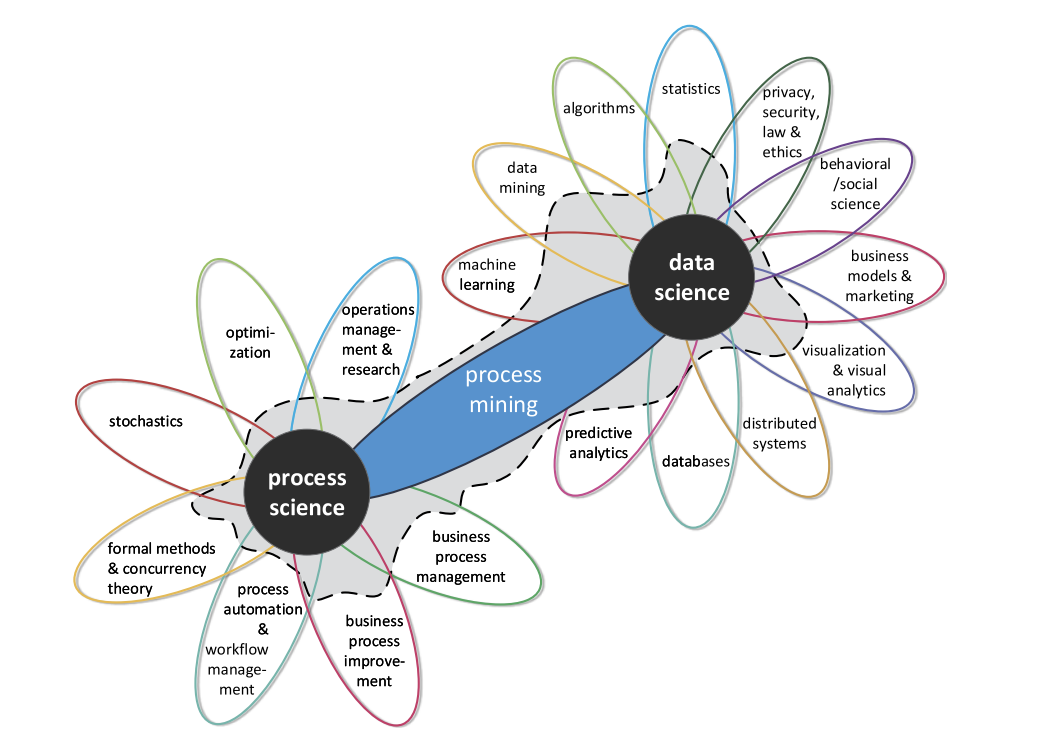
\includegraphics[width=1\textwidth]{images/3.methodology/process_mining.png}
    \caption[Process Mining as an interdisciplinary Discipline]{Process Mining as an interdisciplinary Discipline \textsuperscript{1}}
    \label{fig:process_mining}
\end{figure}

\addtocounter{footnote}{1}
\footnotetext[\value{footnote}]{From \textit{Process Mining}(p.18), by Wil van der Aalst, 2016, Berlin, Heidelberg: Springer Berlin Heidelberg. Copyright [2016] by Springer Berlin Heidelberg.}
As depicted in Figure \ref{fig:process_mining}, process mining intersects with domains in data science, including statistics, databases, computational intelligence, data mining, and visual analytics. Simultaneously, it intersects with domains in process science, such as business process management, optimization, stochastics, process automation and workflow management, and operations management and research. Process mining serves as a bridge between data and process science \cite{van_der_aalst_process_2016}.

\subsection*{PM Methodology and Techniques}

A standard methodology for such projects was established by \citeA{van_eck_pm2_2015}, known as the Process Mining Project Methodology.

\begin{figure}[H]
    \centering
    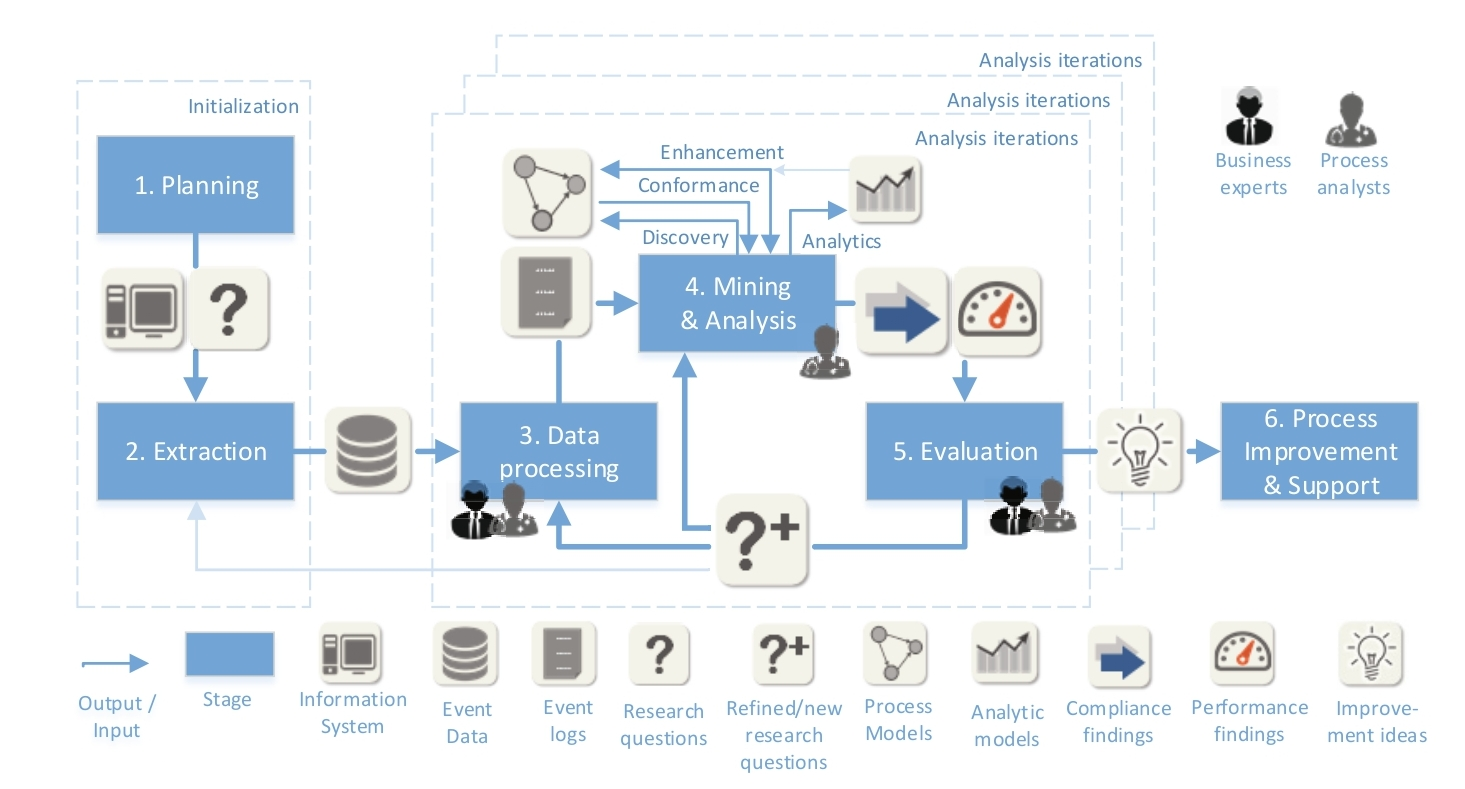
\includegraphics[width=1\textwidth]{images/3.methodology/process_mining_methodology.jpg}
    \caption[Overview of the Process Mining Project Methodology]{Overview of the Process Mining Project Methodology \textsuperscript{1}}
    \label{fig:process_mining_methodology}
\end{figure}

\footnotetext[\value{footnote}]{From \textit{PM\textsuperscript{2}: A Process Mining Project Methodology}(p.299), by van Eck et al., 2015, Cham, Springer International Publishing. Copyright [2015] by Springer International Publishing.}

Each stage depicted in Figure \ref{fig:process_mining_methodology} is carefully described by \citeA{van_eck_pm2_2015} in their publication. Here is an overview of each stage as described by them:

\begin{quote}
\textit{The first two stages of the methodology are (1) planning and (2) extraction, during which initial research questions are defined and event data are extracted. After the first two stages, one or more analysis iterations are performed, possibly in parallel. In general, each analysis iteration executes the following stages one or more times: (3) data processing, (4) mining \& analysis, and (5) evaluation. An analysis iteration focusses on answering a specific research question by applying process mining related activities and evaluating the discovered process models and other findings. Such an iteration may take anywhere from minutes to days to complete, mainly depending on the complexity of the mining \& analysis. If the findings are satisfactory then they can be used for (6) process improvement \& support.}
\end{quote}

\begin{figure}[H]
    \centering
    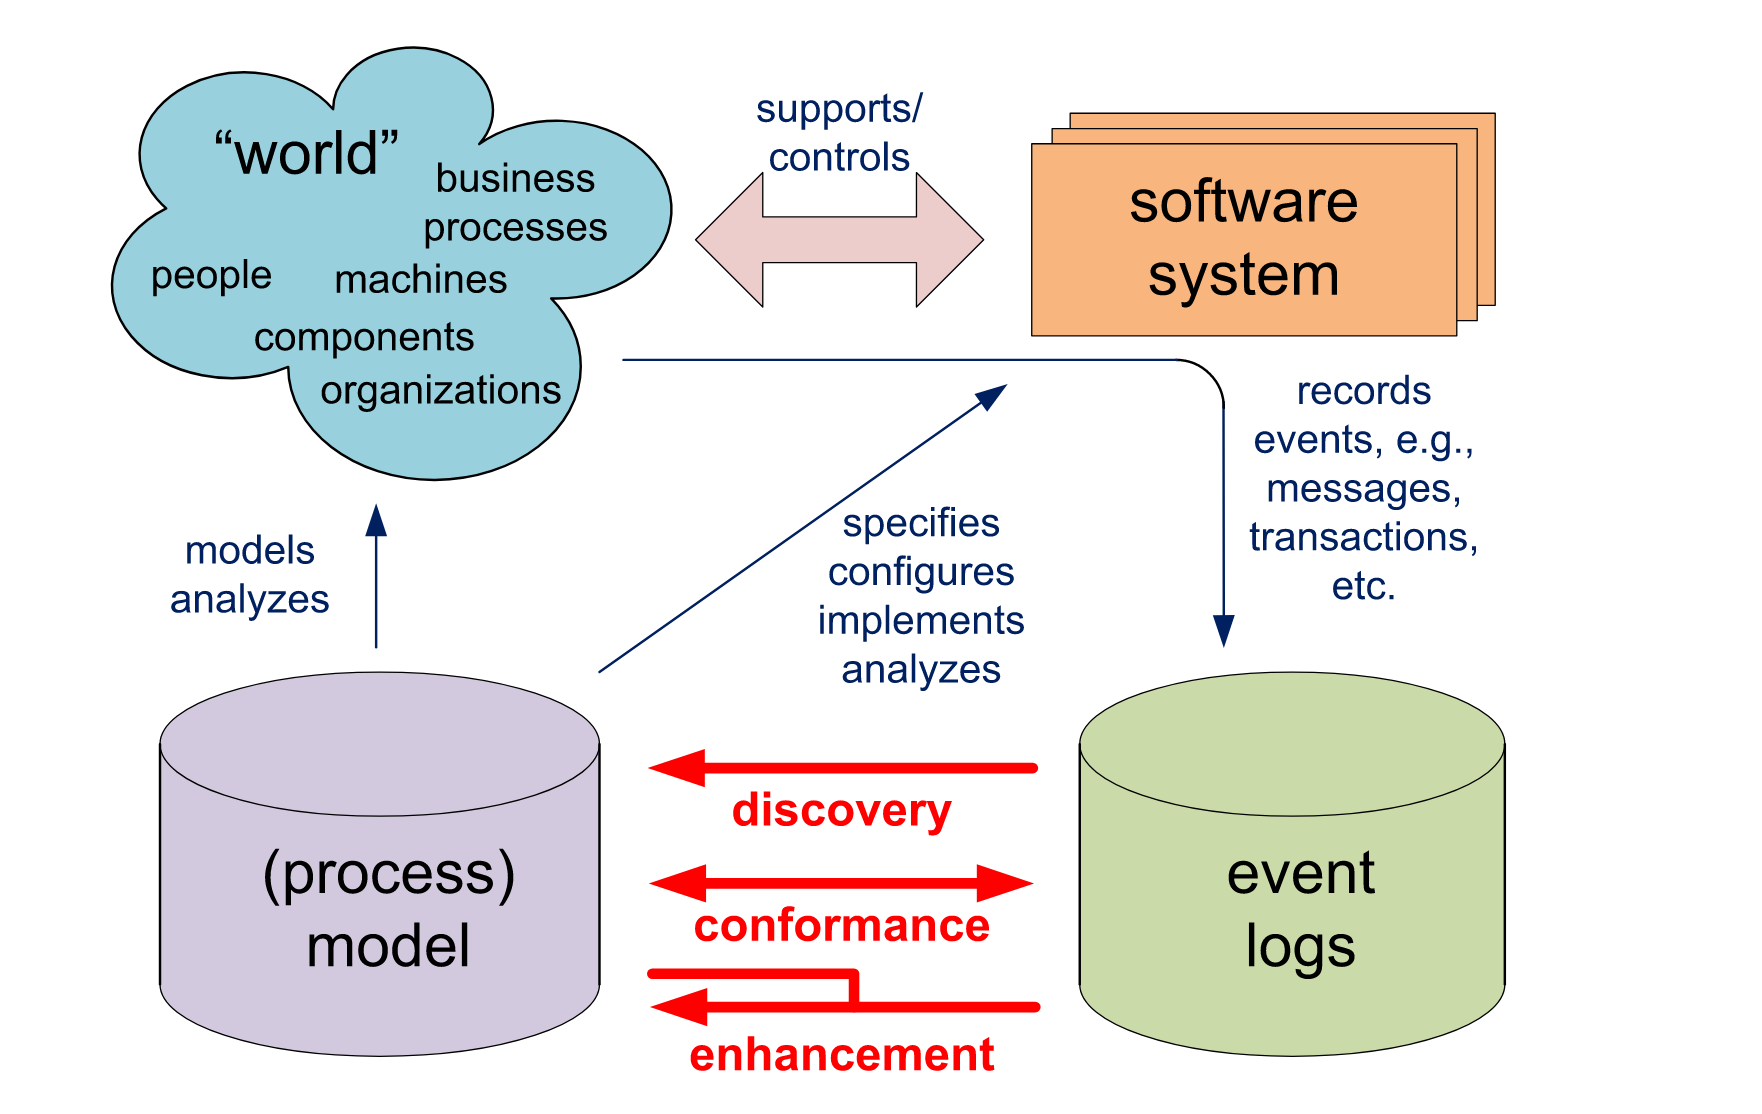
\includegraphics[width=1\textwidth]{images/3.methodology/process_mining_techniques.png}
    \caption[Process Mining Techniques]{Process Mining Techniques \textsuperscript{1}}
    \label{fig:process_mining_techniques}
\end{figure}

\footnotetext[\value{footnote}]{From \textit{Process Mining}(p.32), by Wil van der Aalst, 2016, Berlin, Heidelberg: Springer Berlin Heidelberg. Copyright [2016] by Springer Berlin Heidelberg.}

As depicted in Figure \ref{fig:process_mining_techniques}, the core techniques in PM consist of Process Discovery, Conformance Checking, and Process Enhancement. Process Discovery involves extracting process models from a log, while Conformance Checking examines deviations by comparing the model and log. Process Enhancement extends or refines existing models using a log. In this study, our focus was exclusively on Process Discovery. This decision was made by the absence of a rigorous model depicting the Stage or Benefits process, rendering Conformance Checking pointless. Additionally, as process enhancements were guided by professional recommendations rather than the refinement of an existing model, the Process Enhancement technique was also considered impractical.

\subsection*{Specialized Methodology for Exploring CRC Care Processes}

While standard methodologies and techniques provide a broad understanding of typical PM projects, this study employed a specific approach tailored to its objectives. The primary aim of PM in this study was to explore the CRC care process through Process Discovery. To achieve this, we utilized a specialized methodology developed by \citeA{vathy-fogarassy_multi-level_2022}, known as the Process Mining Methodology for Exploring Disease-specific Care Processes (MEDCP).

This methodology is designed to address the intricacies of exploring disease-specific care processes by working at different levels of abstraction. It involves preprocessing the data to group detailed activities into higher event groups, allowing researchers to view activities from a simplified perspective without ignoring less frequently traveled pathways.

\begin{figure}[H]
    \centering
    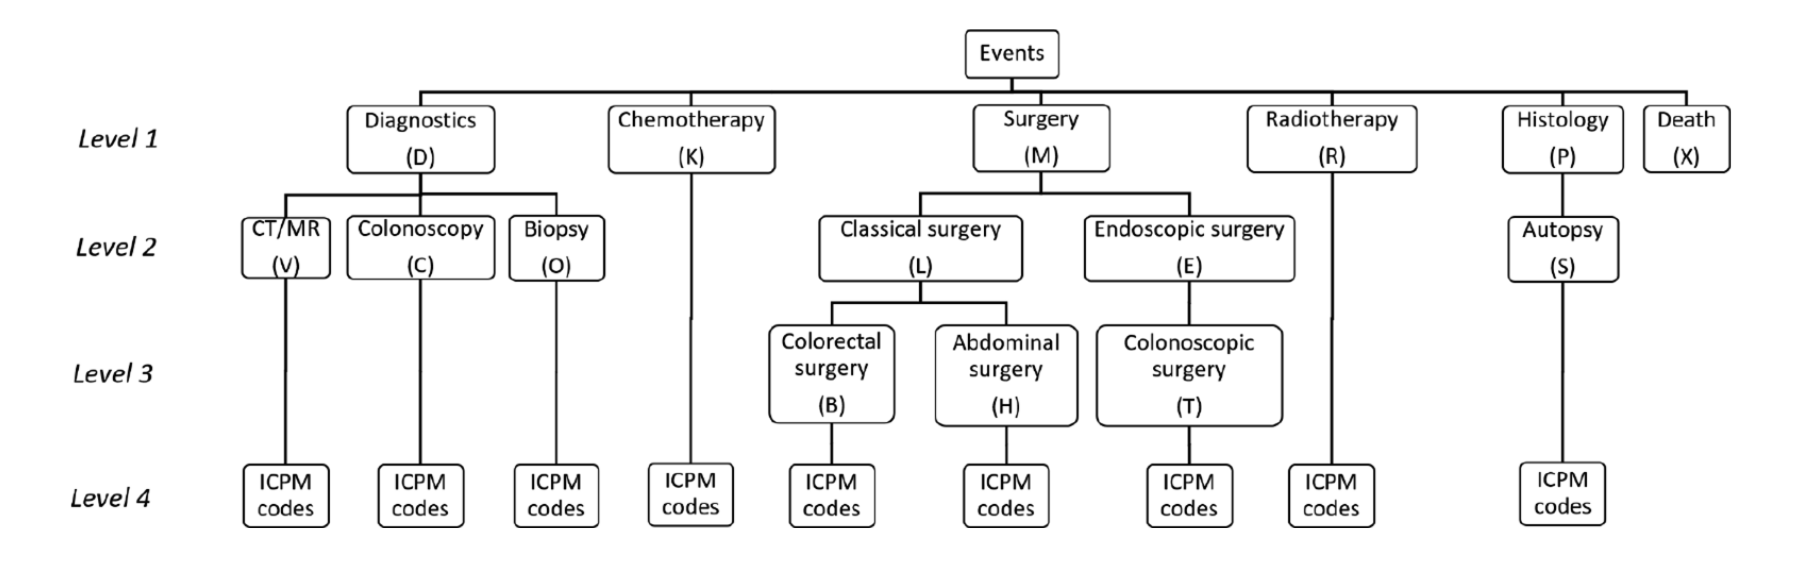
\includegraphics[width=1\textwidth]{images/3.methodology/MEDDCP_CRC_case.png}
    \caption[CRC Multi-level Abstraction]{CRC Multi-level Abstraction\textsuperscript{1}}
    \label{fig:crc_case}
\end{figure}

\footnotetext[\value{footnote}]{From \textit{Multi-level process mining methodology for exploring disease-specific care processes}(p.8), by Vathy-Fogarassy, 2022, Hungary, Jorunal of Biomedical Informatics Copyright [2022] by Journal of Biomedical Informatics.}

As depicted in Figure \ref{fig:crc_case}, for the CRC case detailed by \citeA{vathy-fogarassy_multi-level_2022} in their publication, the methodology organizes interventions into four levels: detailed procedures into Level 4, surgeries into Level 3, main procedures into Level 2, and main stages of CRC care into Level 1.

This approach proved invaluable, particularly in the selection and preprocessing of data, as it addressed many of the challenges encountered by the researcher. Furthermore, the separation of benefits and stages within the datasets facilitated multi-level abstraction, providing a comprehensive view of the CRC care process in two levels.

\subsection*{The Software of Choice}

For this study, Disco (\href{www.fluxicon.com}{www.fluxicon.com}) was selected as the software of choice from a range of Process Mining tools, including ProM (\href{www.promtools.org}{www.promtools.org}) and Celonis (\href{www.celonis.com}{www.celonis.com}), all of which the researcher is familiar with. Disco proved to be the optimal solution due to its user-friendly interface and robust functionality. Its intuitive design facilitated seamless data import and visualization, simplifying the exploration of complex process models. Additionally, Disco's comprehensive range of analysis features enabled thorough examination of the CRC care pathway within the SMPHS. Its efficient handling of large datasets proved instrumental in managing the extensive healthcare data required for this investigation. Overall, Disco's combination of accessibility, versatility, and performance made it the ideal choice for conducting Process Mining analysis in this research endeavor.

Next, we will outline the key features of the Disco software.

\begin{figure}[H]
    \centering
    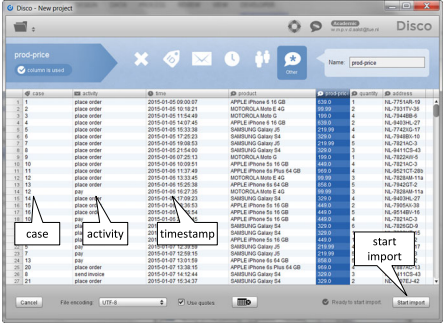
\includegraphics[width=1\textwidth]{images/3.methodology/disco_import.png}
    \caption{Importing a File in Disco}
    \label{fig:disco_importing_file}
\end{figure}

As depicted in Figure \ref{fig:disco_importing_file}, the process of importing files into the system is straightforward. Simply choose the file and indicate which columns will serve as the Case ID, Activity, and Timestamp for both the start and end of each activity. After selecting to start the import, a process map will be displayed.

\begin{figure}[H]
    \centering
    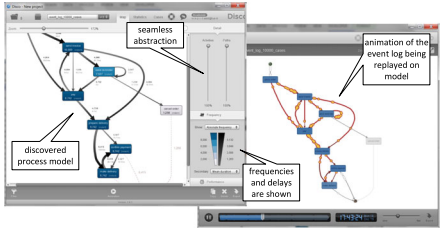
\includegraphics[width=1\textwidth]{images/3.methodology/disco_features.png}
    \caption{Main Disco Features}
    \label{fig:disco_features}
\end{figure}

As depicted in the left image of Figure \ref{fig:disco_features}, the software interface features a process map displayed on the left side. The seamless abstraction panel, positioned at the top right, enables users to adjust the visibility of Activities and Paths within the discovered process model or process map. Additionally, the Frequency and Performance panel located in the bottom right corner of the screen enables users to switch between these two modes, although the Performance mode will not be utilized in this study. Furthermore, users can utilize the Animation panel at the bottom to visualize how individuals behave within the process map, as depicted in the right image of Figure \ref{fig:disco_features}.

\subsection*{Illustrative Example}

When initiating a new project, the initial process map often becomes overwhelming when all activities and paths are included, resulting in what is commonly referred to as "spaghetti maps" due to their complex and tangled appearance.

\begin{figure}[H]
    \centering
    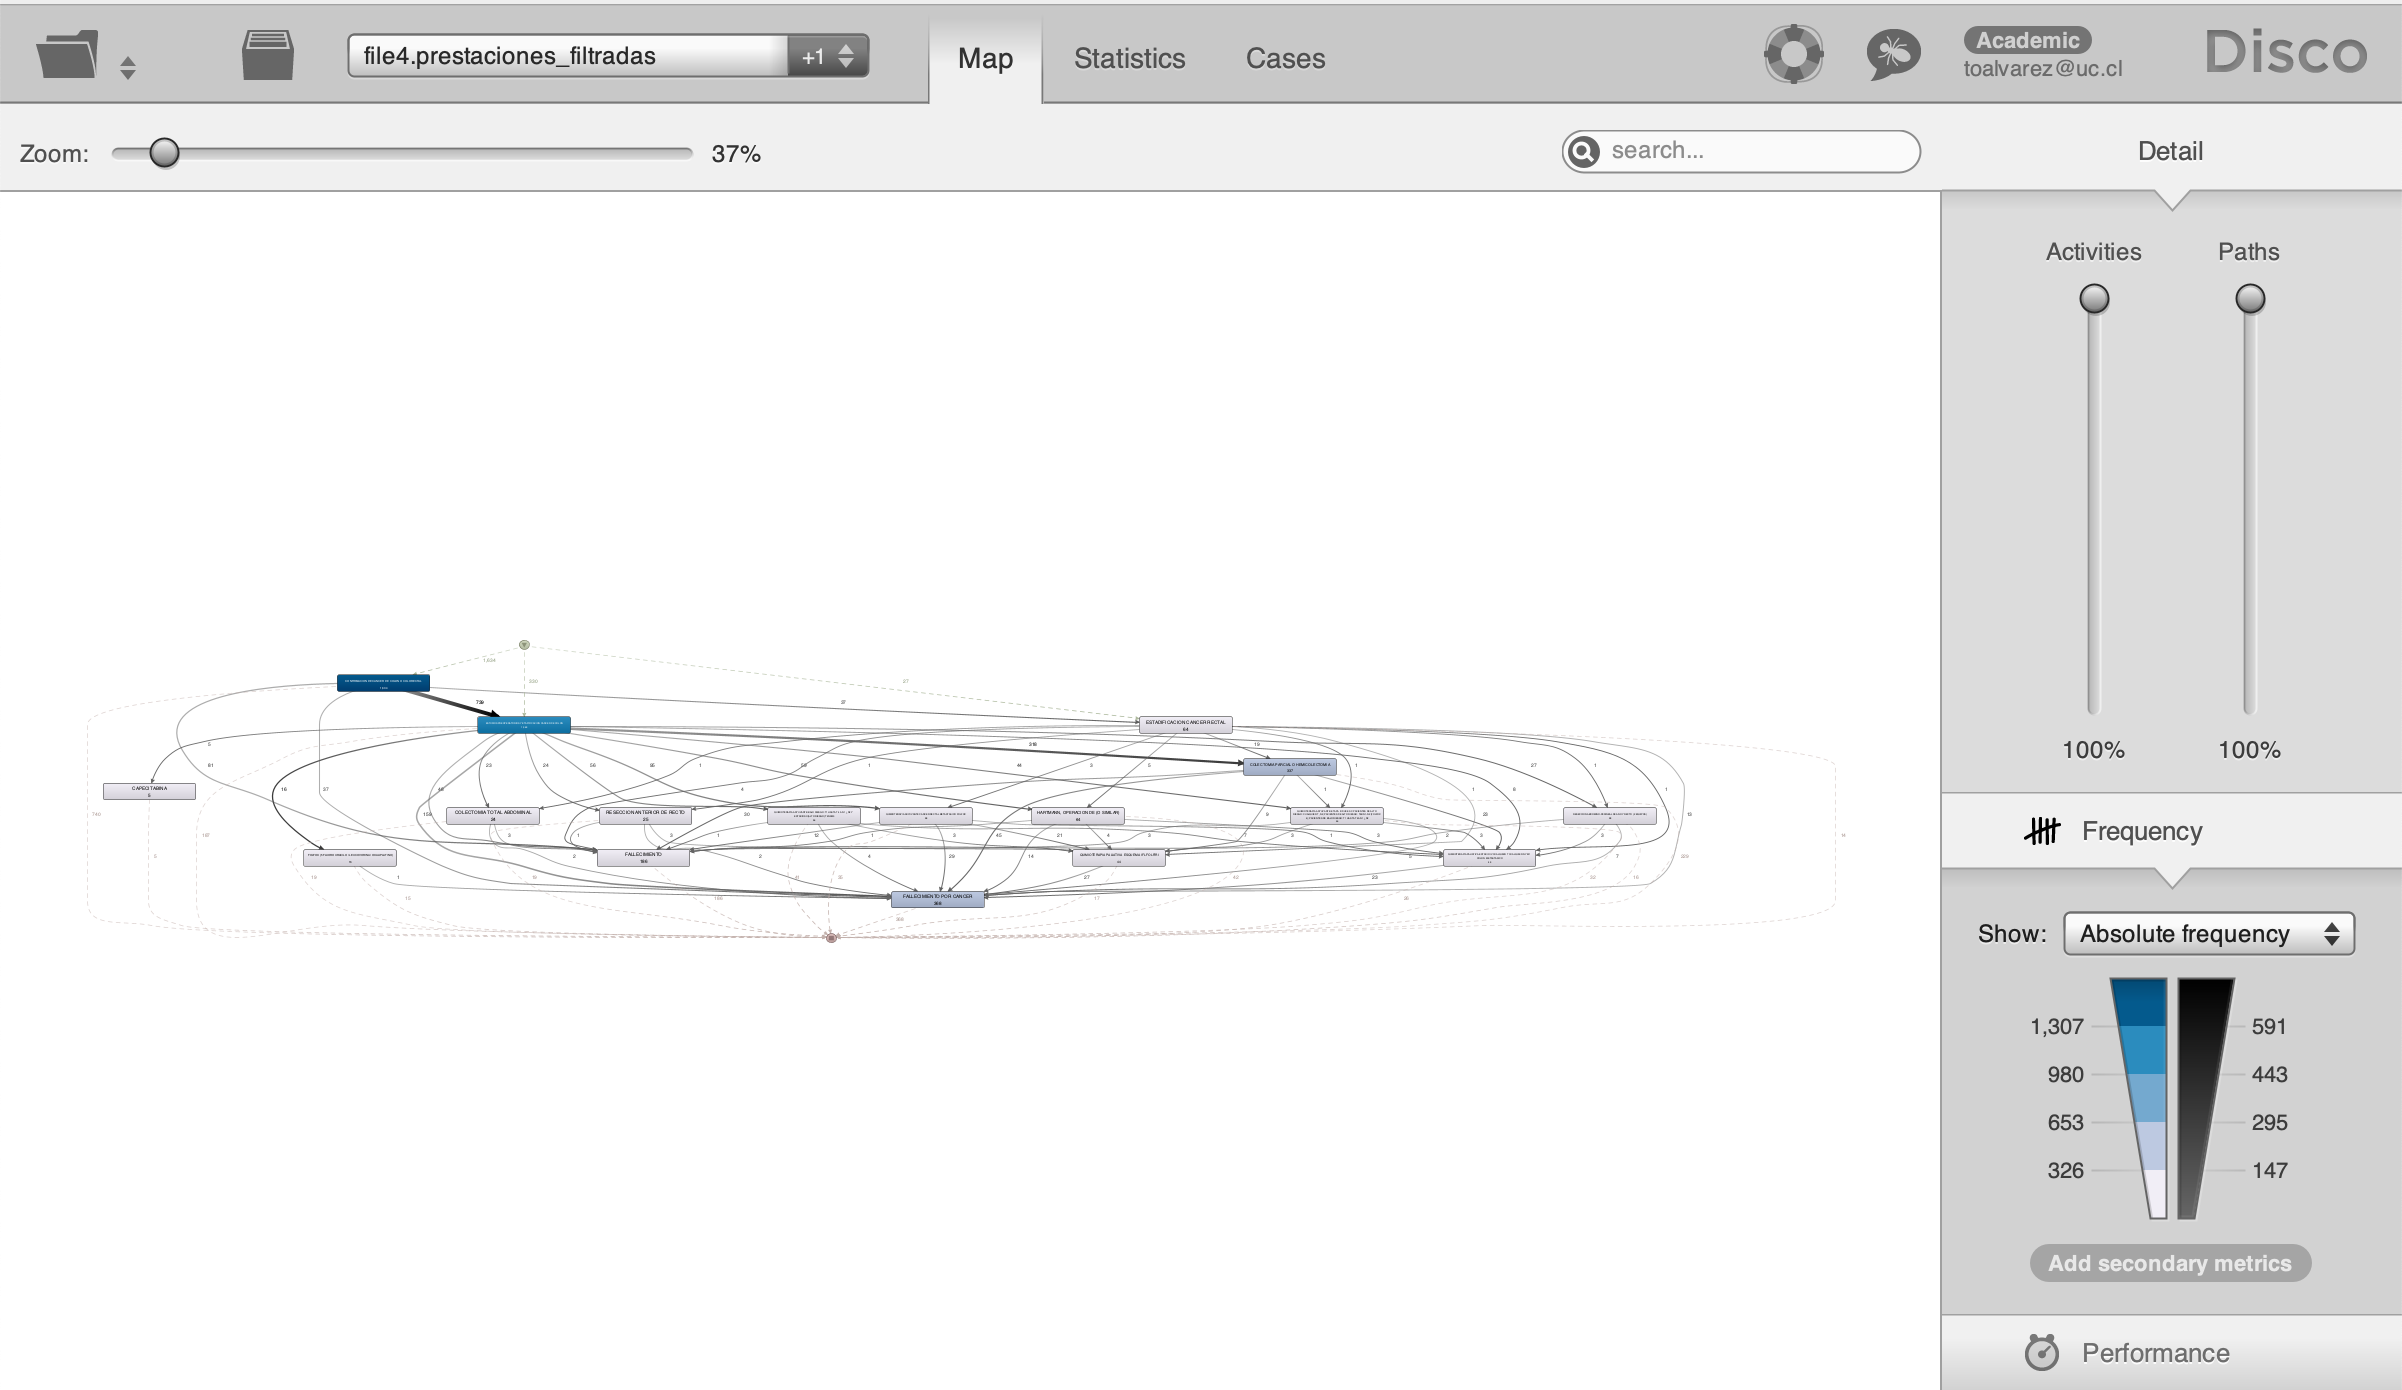
\includegraphics[width=1\textwidth]{images/3.methodology/disco_example_1.png}
    \caption{Disco Benefits Example}
    \label{fig:disco_example_1}
\end{figure}

For instance, Figure \ref{fig:disco_example_1} presents a spaghetti map depicting the Benefits process of CRC patients. To enhance readability, the number of paths has been reduced to approximately 20\% of the most common paths.

\begin{figure}[H]
    \centering
    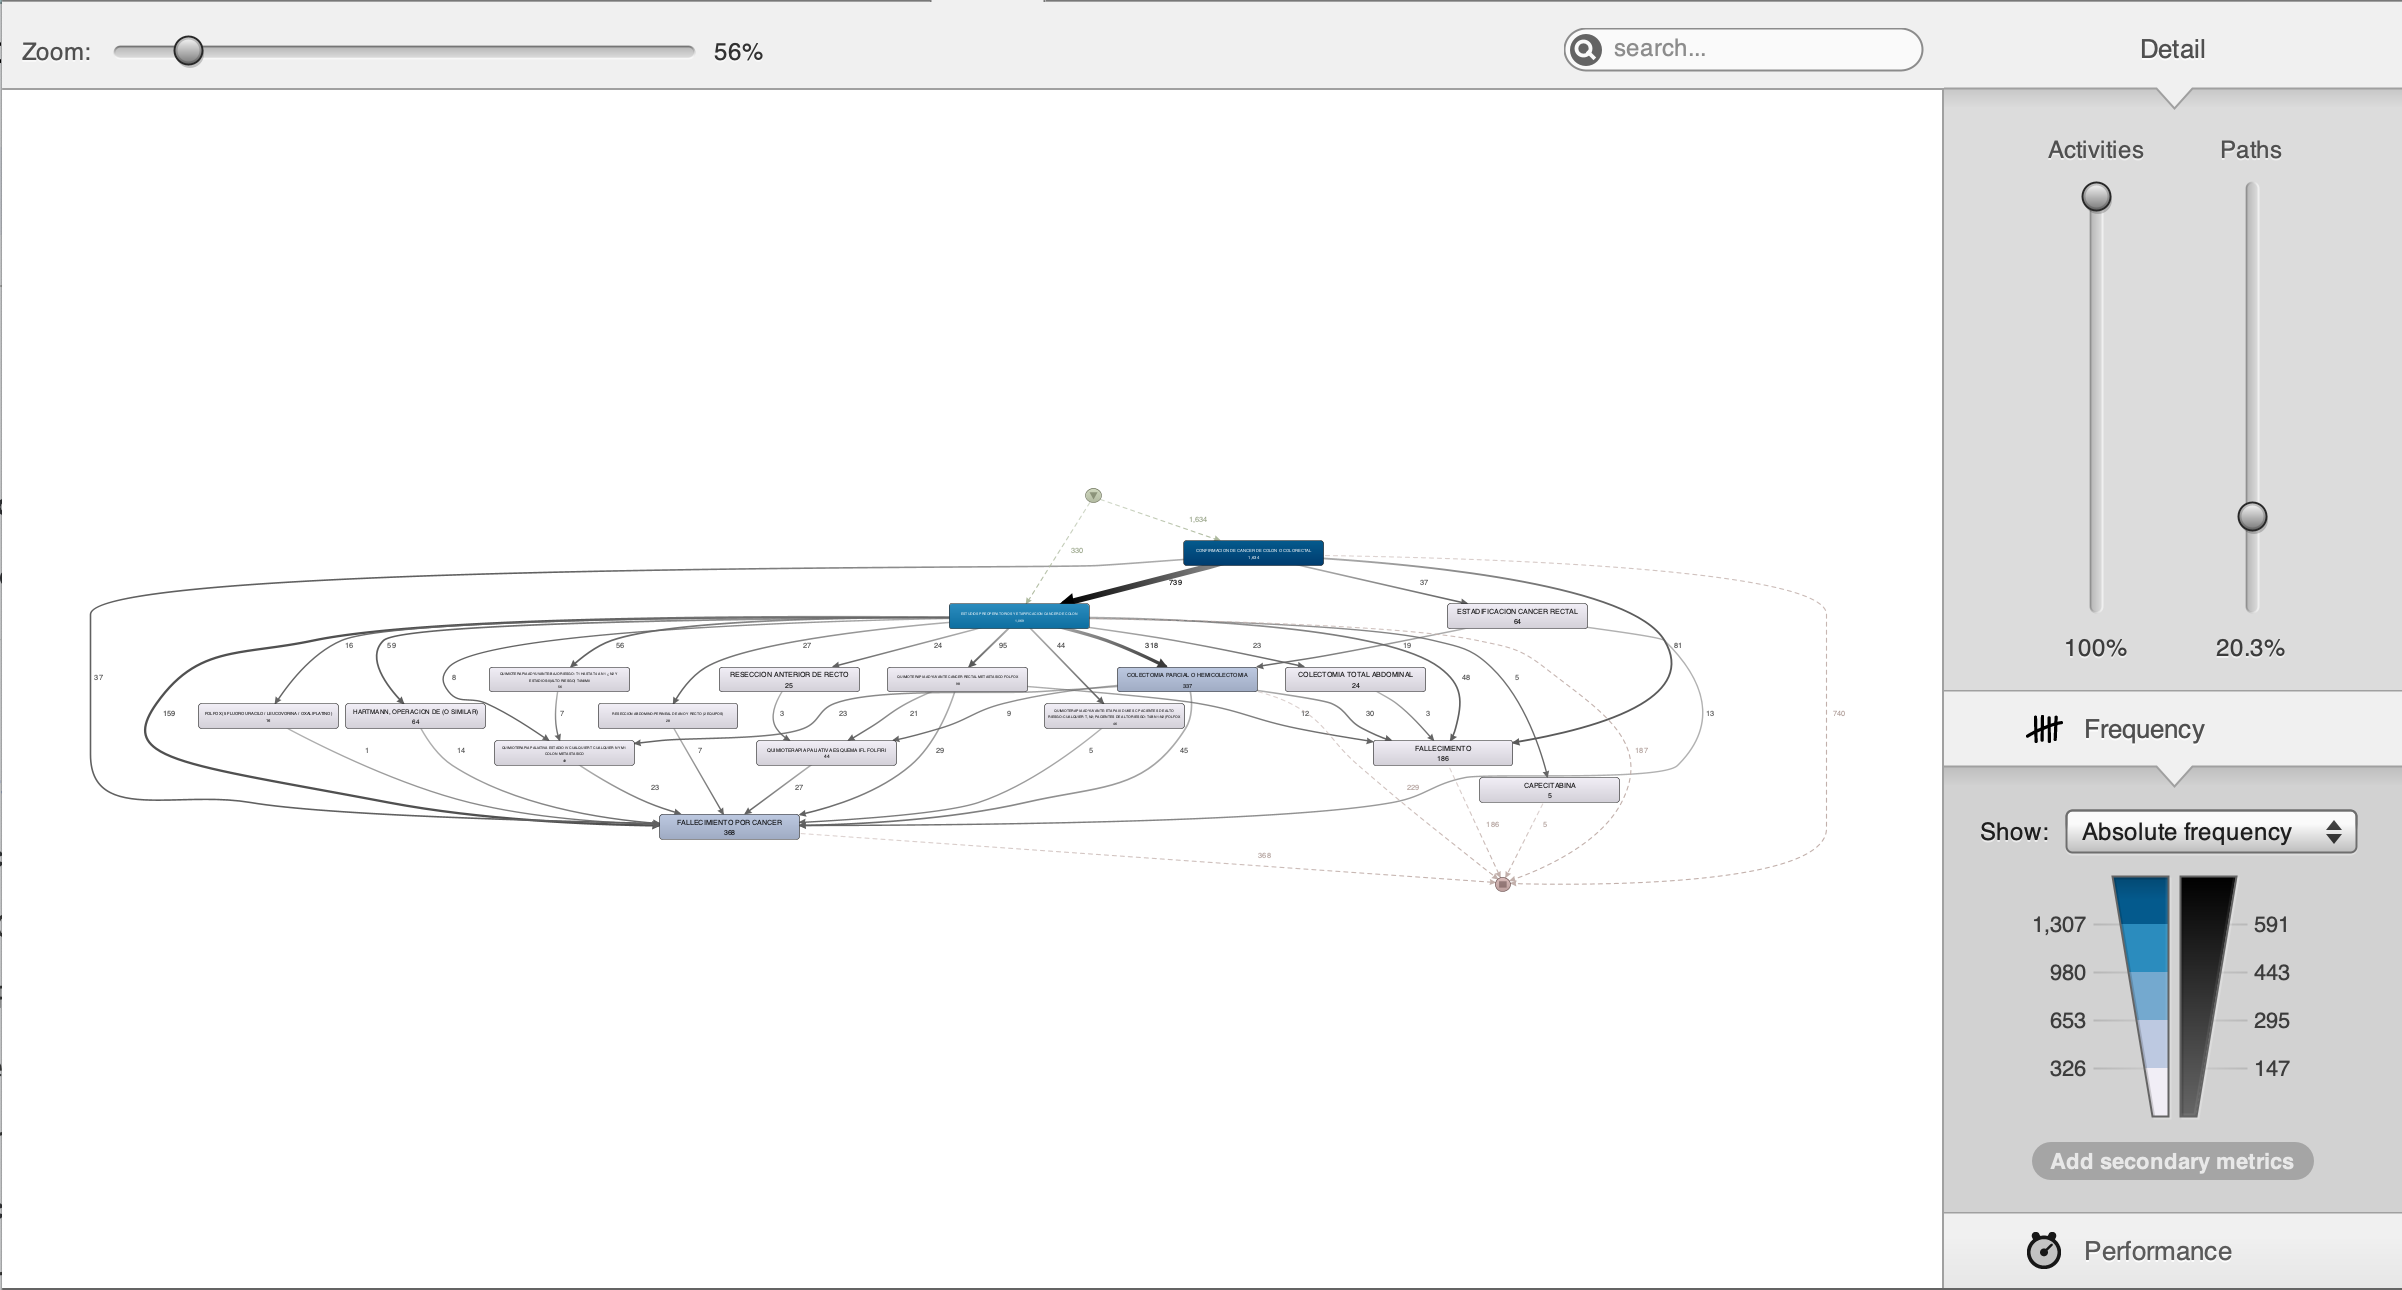
\includegraphics[width=1\textwidth]{images/3.methodology/disco_example_2.png}
    \caption{Disco Benefits Example Activities at 20\%}
    \label{fig:disco_example_2}
\end{figure}

Despite this adjustment, due to the multitude of activities involved, in Figure \ref{fig:disco_example_2} clarity remains a challenge. To address this, the number of activities will also be reduced to around 20\% of the most common activities.

\begin{figure}[H]
    \centering
    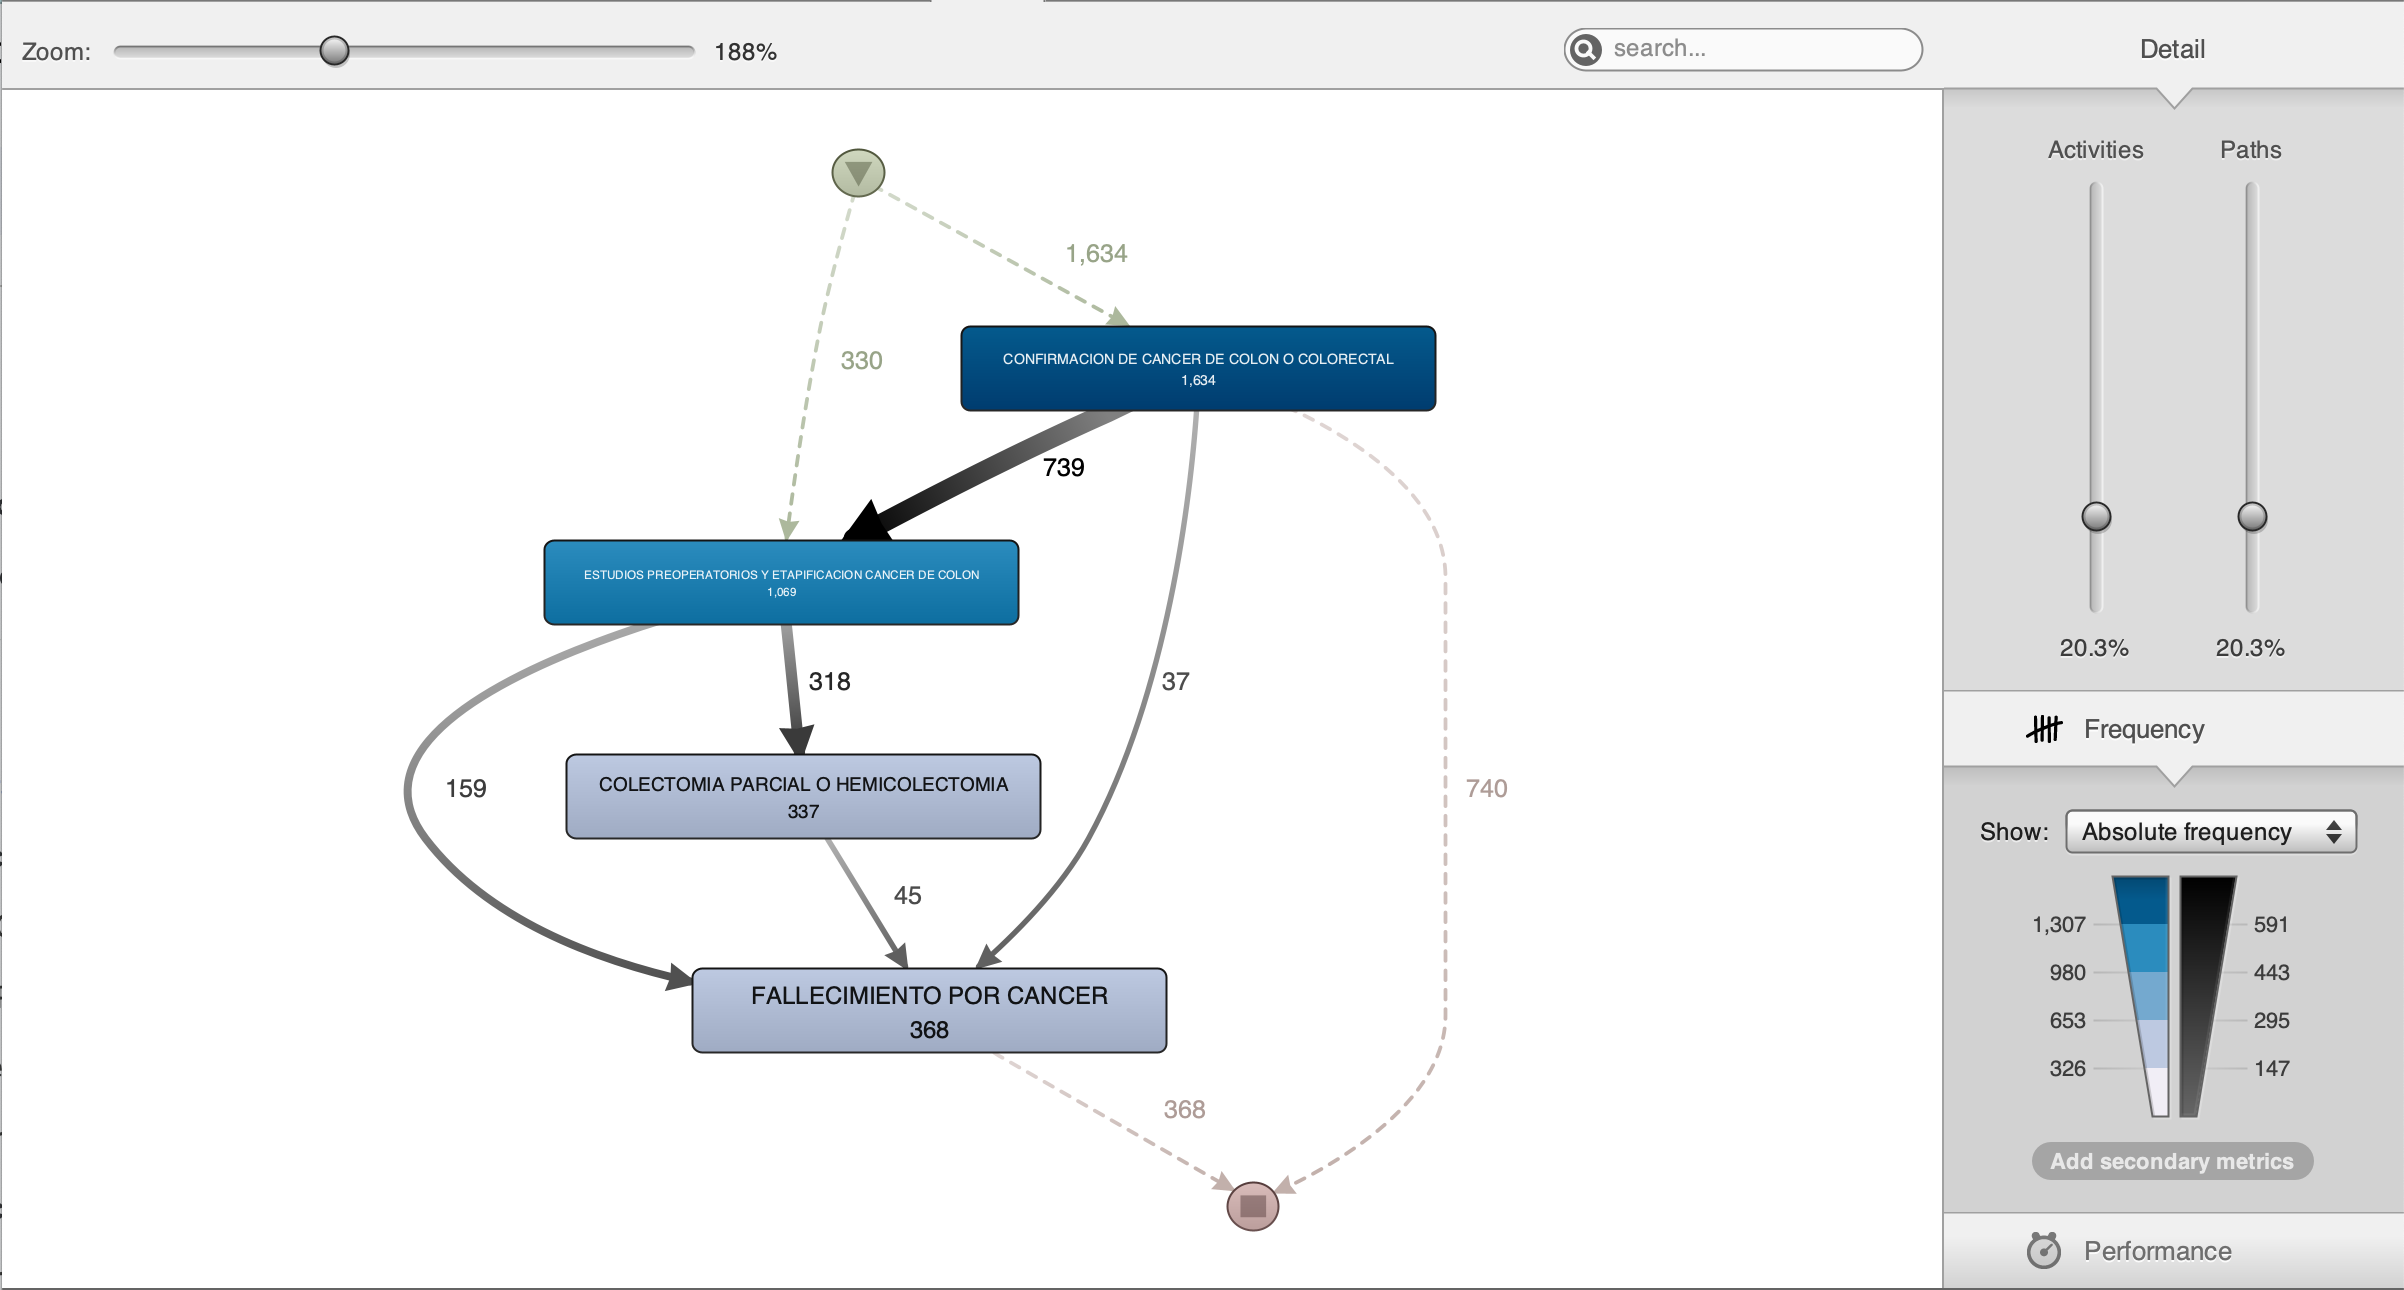
\includegraphics[width=1\textwidth]{images/3.methodology/disco_example_3.png}
    \caption{Disco Benefits Example Activities and Paths at 20\%}
    \label{fig:disco_example_3}
\end{figure}

In the updated Figure \ref{fig:disco_example_3}, we observe a significantly more legible process map. The dominant activity, "CONFIRMACION DE CANCER DE COLON O COLORECTAL" (Confirmation of CRC), appears prominently, occurring 1634 times. The shading of the activities indicates their frequency, with darker color representing higher occurrence. Likewise, the thickness of the arrows representing transitions between activities reflects their frequency. Additionally, the Frequency panel can be adjusted to provide insights into the average duration of each activity transition.

\begin{figure}[H]
    \centering
    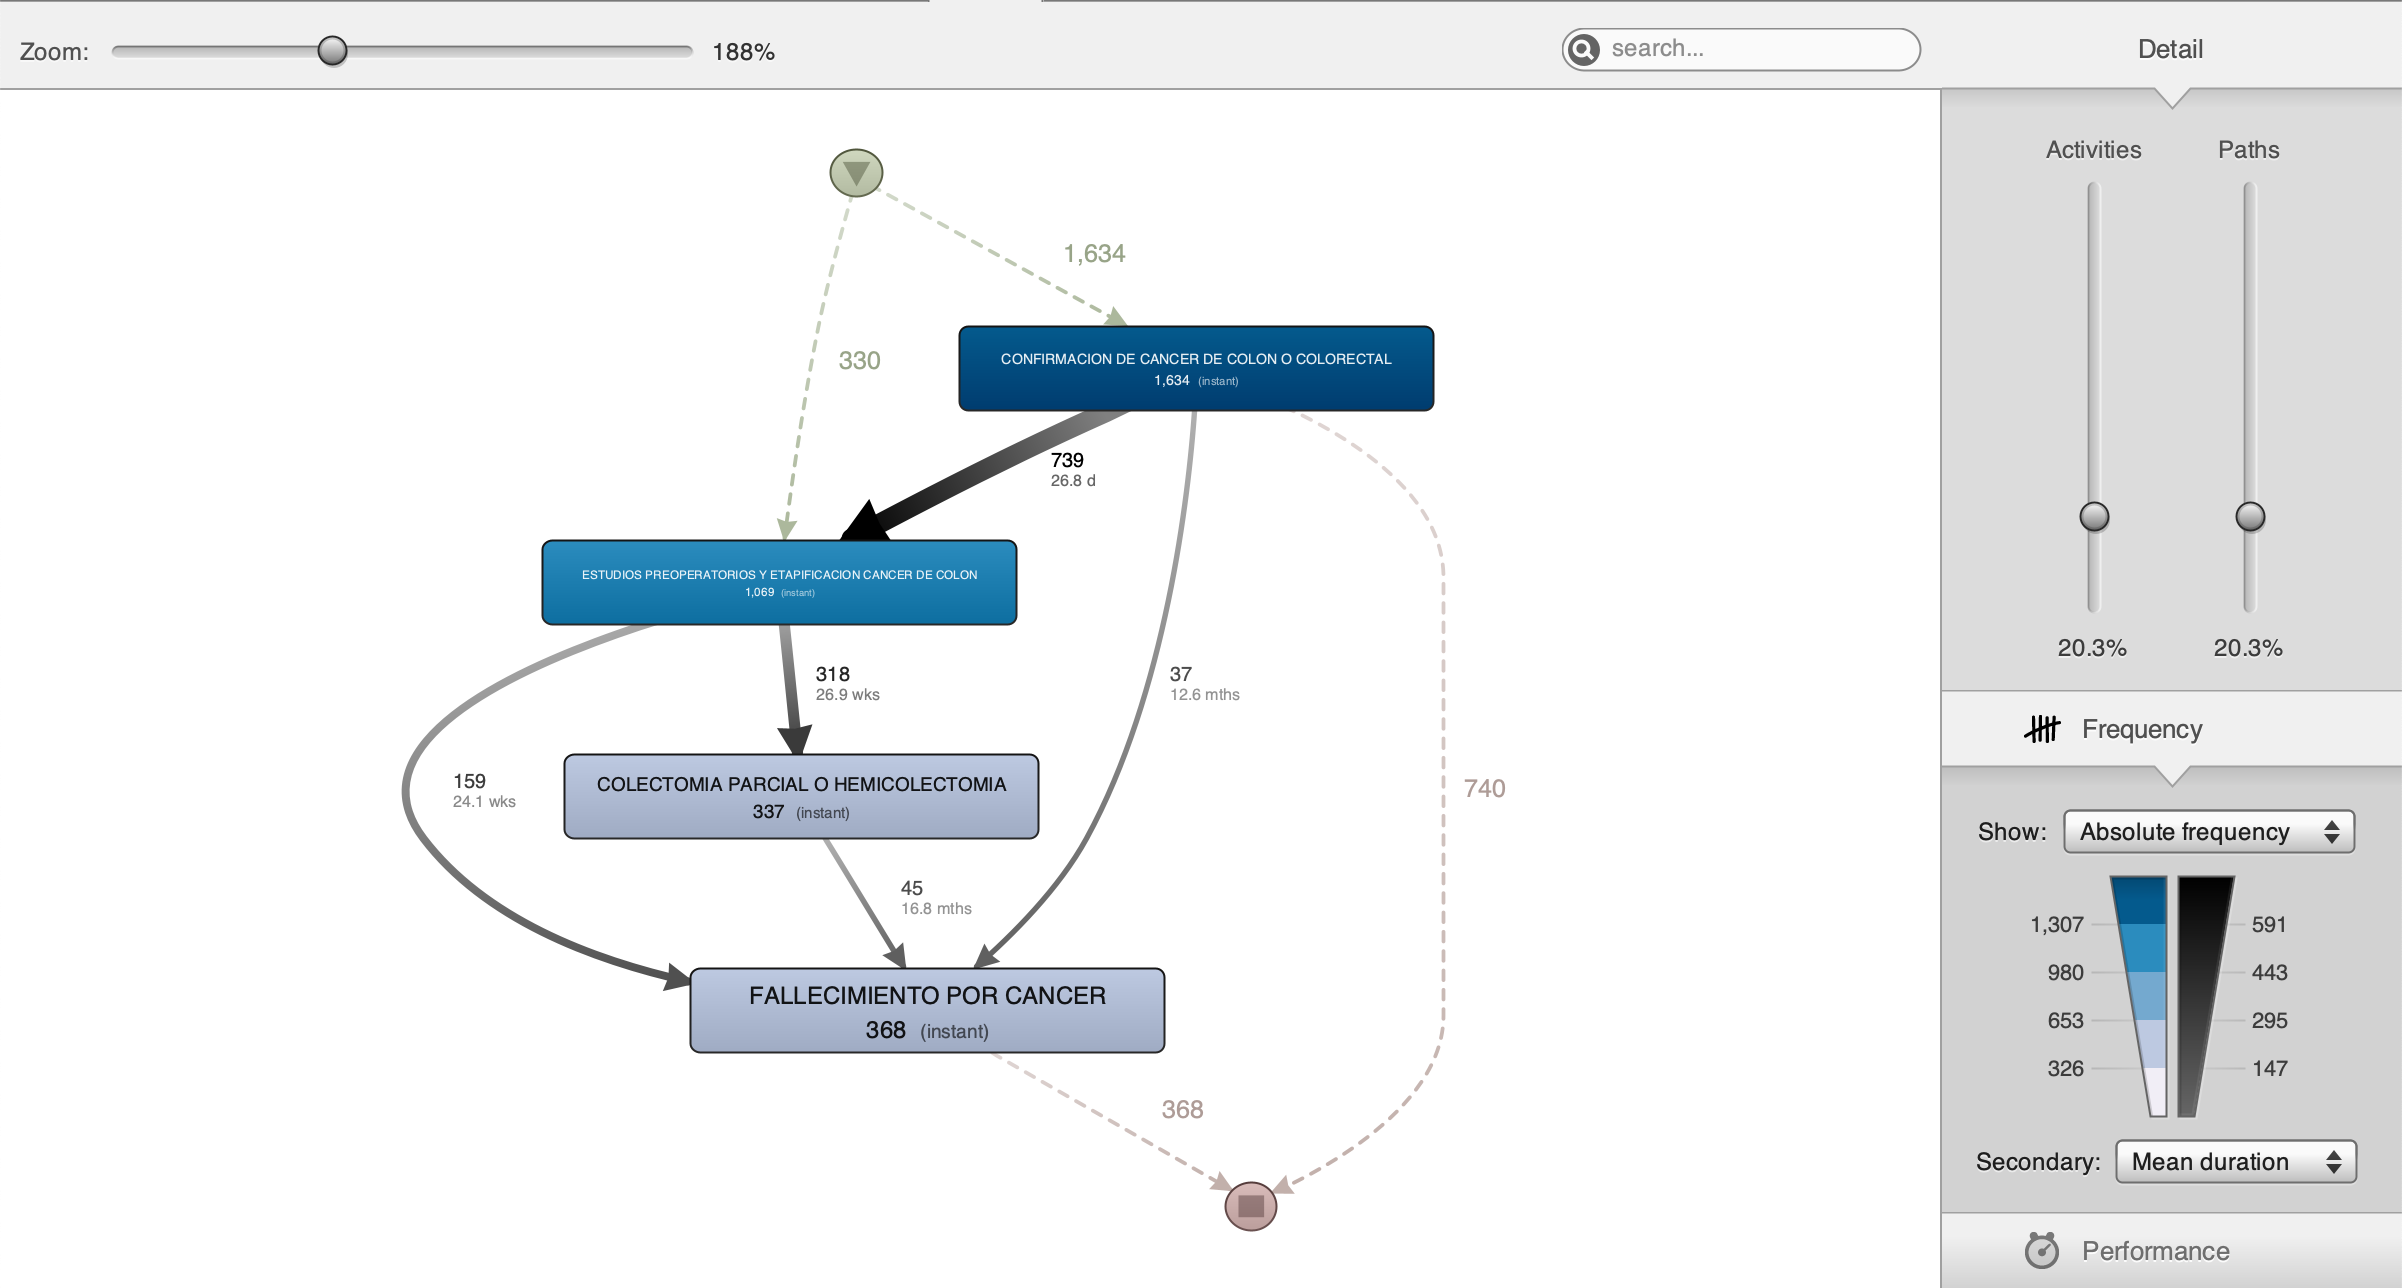
\includegraphics[width=1\textwidth]{images/3.methodology/disco_example_4.png}
    \caption{Disco Benefits Example with Mean Duration}
    \label{fig:disco_example_4}
\end{figure}

Further analysis, as depicted in figure \ref{fig:disco_example_4}, reveals the average transition time between activities. For instance, between "CONFIRMACION DE CANCER DE COLON O COLORECTAL" and "ESTUDIOS PREOPERATORIOS Y ETAPIFICACION CANCER DE COLON" (preoperative evaluation and CRC staging), 739 transitions occurred, with an average duration of 26.8 days. It's important to note that this calculation relies on the availability of timestamps marking the start and, ideally, the end of each activity. In cases where only one timestamp is available, indicating the activity's initiation, the duration is represented as "instant."

\section{Process Discovery}

The process discovery stage adopts the MEDCP methodology described by \citeA{vathy-fogarassy_multi-level_2022}. Initially, data is collected, followed by a meticulous cleaning process to construct event logs, a fundamental prerequisite for process mining analysis. Subsequently, the refined event logs are used to initiate process discovery through the process maps generated by the selected software. Furthermore, insights from the MND team are incorporated to deepen the understanding of the CRC care process. Lastly, performance metrics are introduced to offer additional insights for the process analysis.
\subsection*{Data Collection}

The data collected is primarily sourced from the comprehensive information cataloged by the SIGGES program. This government initiative, integral to monitoring benefits under the Explicit Guarantees in Health (GES) program, guarantees access to specific healthcare exams and treatments for a predetermined list of prevalent diseases. Two comprehensive datasets were provided by the MND team to support this research. 

\begin{figure}[H]
    \centering
    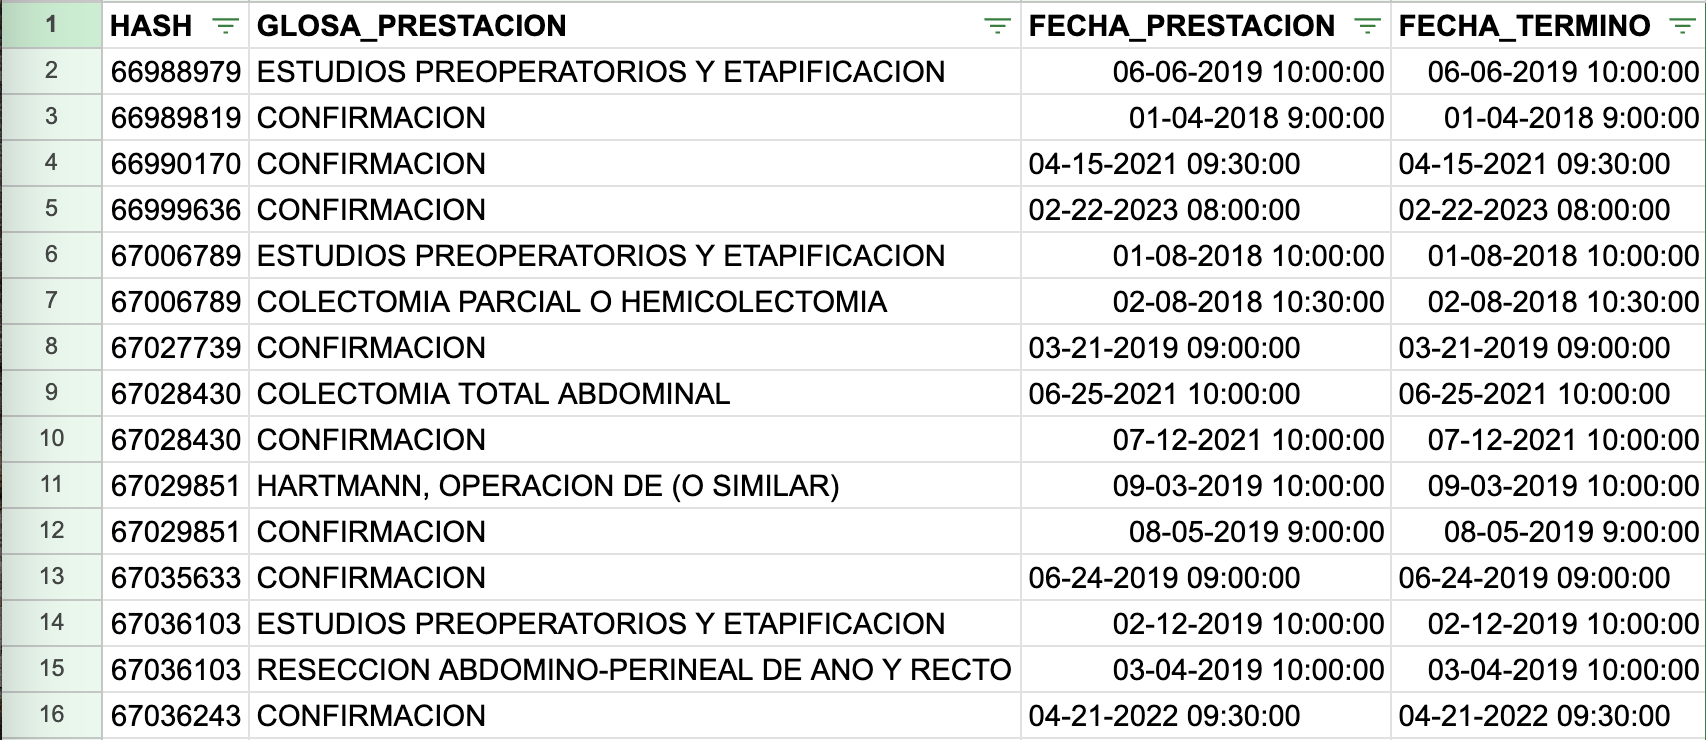
\includegraphics[width=1\textwidth]{images/3.methodology/benefits_dataset.png}
    \caption{Benefits Dataset}
    \label{fig:benefits_dataset}
\end{figure}

As depicted in Figure \ref{fig:benefits_dataset}, the first dataset meticulously outlines the specific benefits of the GES program accessed by each patient in the district over a five-year period, offering a detailed view of each patient's journey with the disease. However, a limitation of this dataset lies in its provision of only the initiation date for each benefit.

\begin{figure}[H]
    \centering
    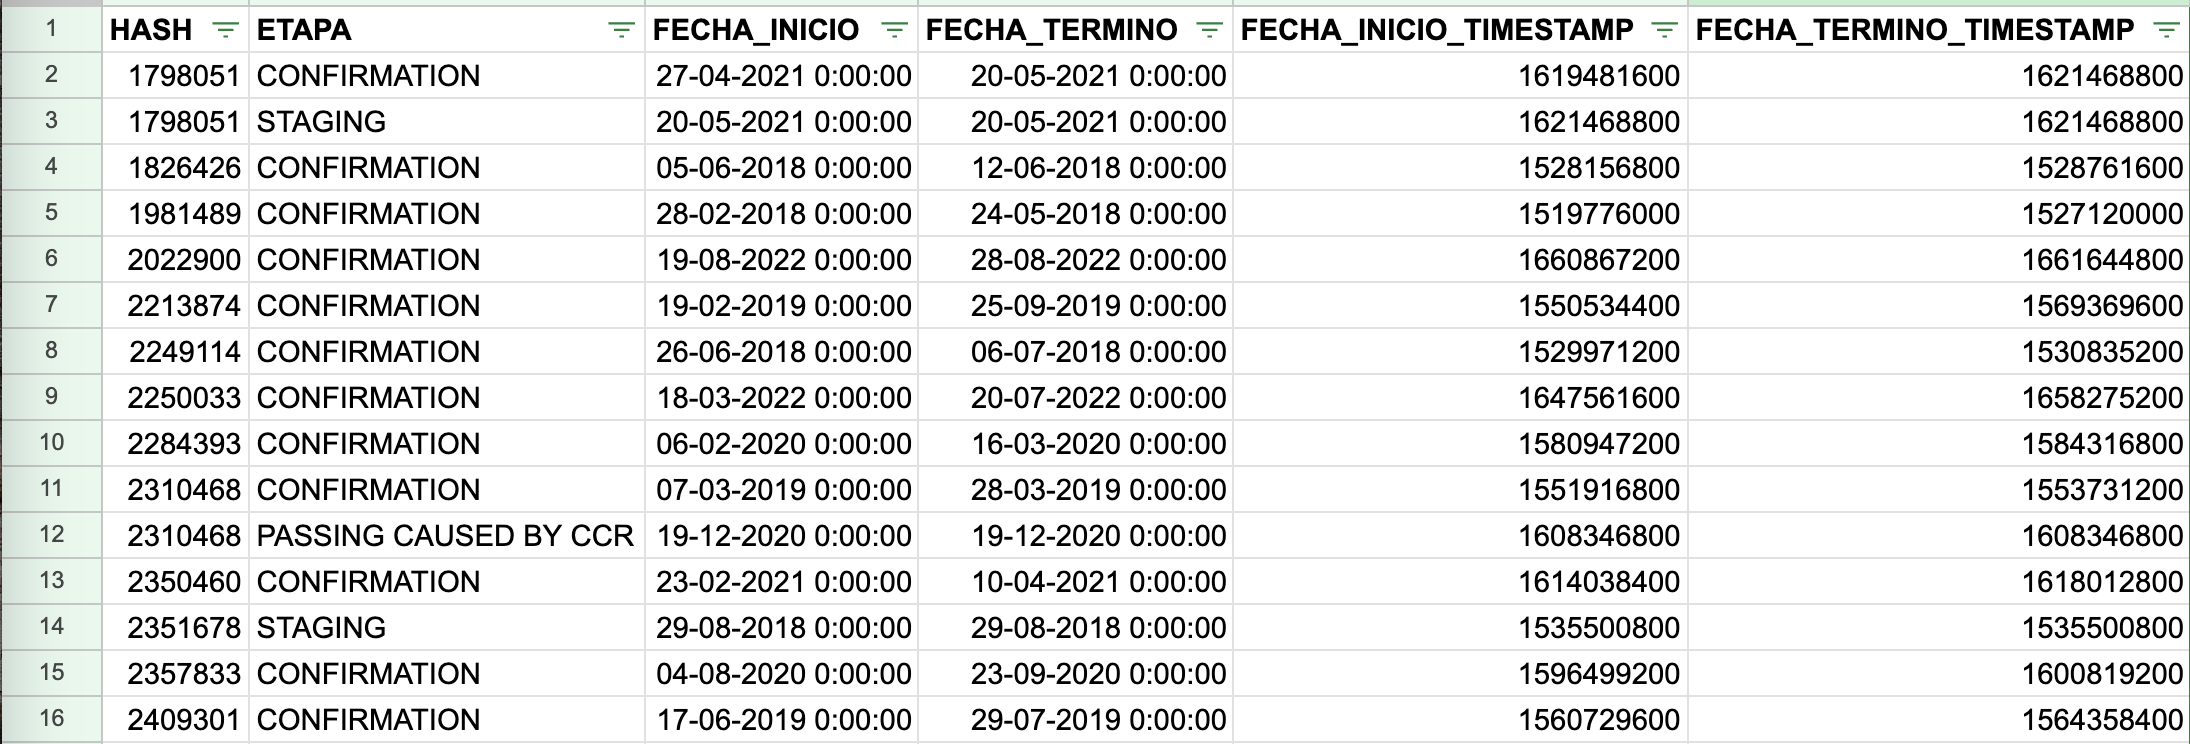
\includegraphics[width=1\textwidth]{images/3.methodology/stages_dataset.png}
    \caption{Stages Dataset}
    \label{fig:stages_dataset}
\end{figure}

In contrast, as seen in Figure \ref{fig:stages_dataset}, the second dataset focuses specifically on the stages undergone by patients during their diagnosis and treatment of CRC in a six-year period, covering confirmation, staging, and treatment phases. This dataset provides both the start and end dates for each stage, enabling the calculation of the duration of each phase.


\begin{table}[H]
\caption{Original Database Overview}
\centering
\begin{tabular}{|c|c|c|c|c|}
\hline
DB & Patients & Source & Initial Data & Final Date\\ \hline
GES Benefits & 3648 & SIGGES & 12/03/2013 & 19/05/2023\\ \hline
GES Stages & 2989 & SIGGES & 4/10/2017  & 23/09/2023\\ \hline
\end{tabular}
\label{table:original_database_overview}
\end{table}


As indicated in Table \ref{table:original_database_overview}, each dataset contains a sufficient number of patients to perform a successful PM analysis. This suggests that the SIGGES database can easily support a two-level abstraction approach for studying each disease using PM.

The second dataset included information regarding the deaths of individuals, with distinctions made between those associated with CRC and those resulting from other causes. This additional information, vital for a comprehensive understanding, was extracted from the cause of death records within the government's databases, ensuring the inclusion of patient mortality data in our analysis.

\label{sec:data_preprocessing}
\subsection*{Data Preprocessing}

The first step of the process was case and activity filtering based on the rules described in the MEDCP methodology \cite{vathy-fogarassy_multi-level_2022}. 

\begin{itemize}

    \item {Standardized date formats.}

    \item {Separated activities with the same timestamp by a small margin according to their logical order.}

    \item {Stacked activities in the Benefits dataset that were performed in a sequence without interrumption.}

    \item {Removed all activities not related to the diagnosis or treatment of the disease.}

    \item {Deleted events outside of the analysis period.}

    \item {Removed uncommon patient sequences.}

    \item {Removed unimportant treatment and diagnosis events.}
\end{itemize}
 

For the Benefits database, only cases that started before 2023 and had a stage sequence repeated more than 10 times were considered. Additionally, benefits that were delivered more than 40 times and provided since 2018 were included.

For the Stages database, only cases that started before 2023, had a stage sequence repeated more than 10 times, and had their treatment started before 2019 were considered.

The results of this process are shown in Table \ref{table:preprocessed_database_overview}.

\begin{table}[H]
\caption{Preprocessed Database Overview}
\centering
\begin{tabular}{|c|c|c|c|c|}
\hline
DB & Patients & Source & Initial Data & Final Date\\ \hline
GES Benefits & 2048 & SIGGES & 01/01/2018 & 22/09/2023\\ \hline
GES Stages & 2524 & SIGGES & 15/11/2017  & 23/09/2023\\ \hline
\end{tabular}
\label{table:preprocessed_database_overview}
\end{table}

\subsection*{Process Mining Results}

Our initial investigation aims to examine the different stages of the process to identify common pathways and quantify the number of individuals entering and exiting each stage. Figure \ref{fig:stages_in_disco} depicts the process map, encompassing 100\% of the activities and paths.

\begin{figure}[H]
    \centering
    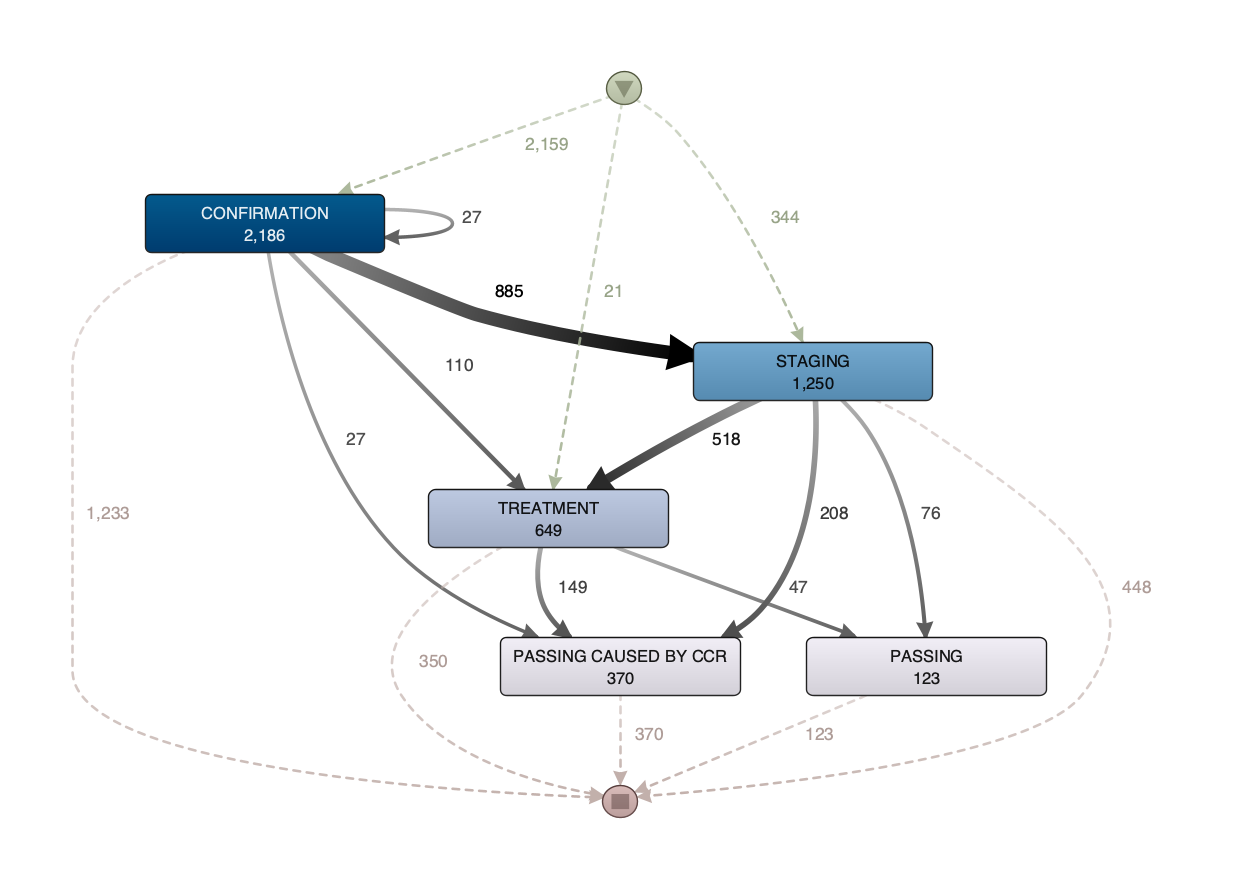
\includegraphics[width=1\textwidth]{images/3.methodology/stagesCRC.png}
    \caption{Stages of CRC in Disco}
    \label{fig:stages_in_disco}
\end{figure}


The process map in Figure \ref{fig:stages_in_disco} provides a compelling visual representation of the patient journey through various stages of care. The majority of patients progress solely to the Confirmation stage, signalling most of them were not confirmed with the disease, as evidenced by the relatively low number of CRC-related passings. Notably, nearly half of these individuals proceed to the Staging stage, indicating a substantial subset of patients being confirmed with CRC. From there, 518 patients advance to the Treatment stage, showing a notable proportion opting for treatment within the public healthcare system. However, it's noteworthy that a portion of patients might opt for alternative avenues, such as seeking care in the private sector or choosing not to undergo treatment at all.

Next, we are going to look into the specific benefits that were given to the patients. Figure \ref{fig:benefits_in_disco} illustrates the process map, encapsulating 100\% of the activities and 20\% of the paths.

\begin{figure}[H]
    \centering
    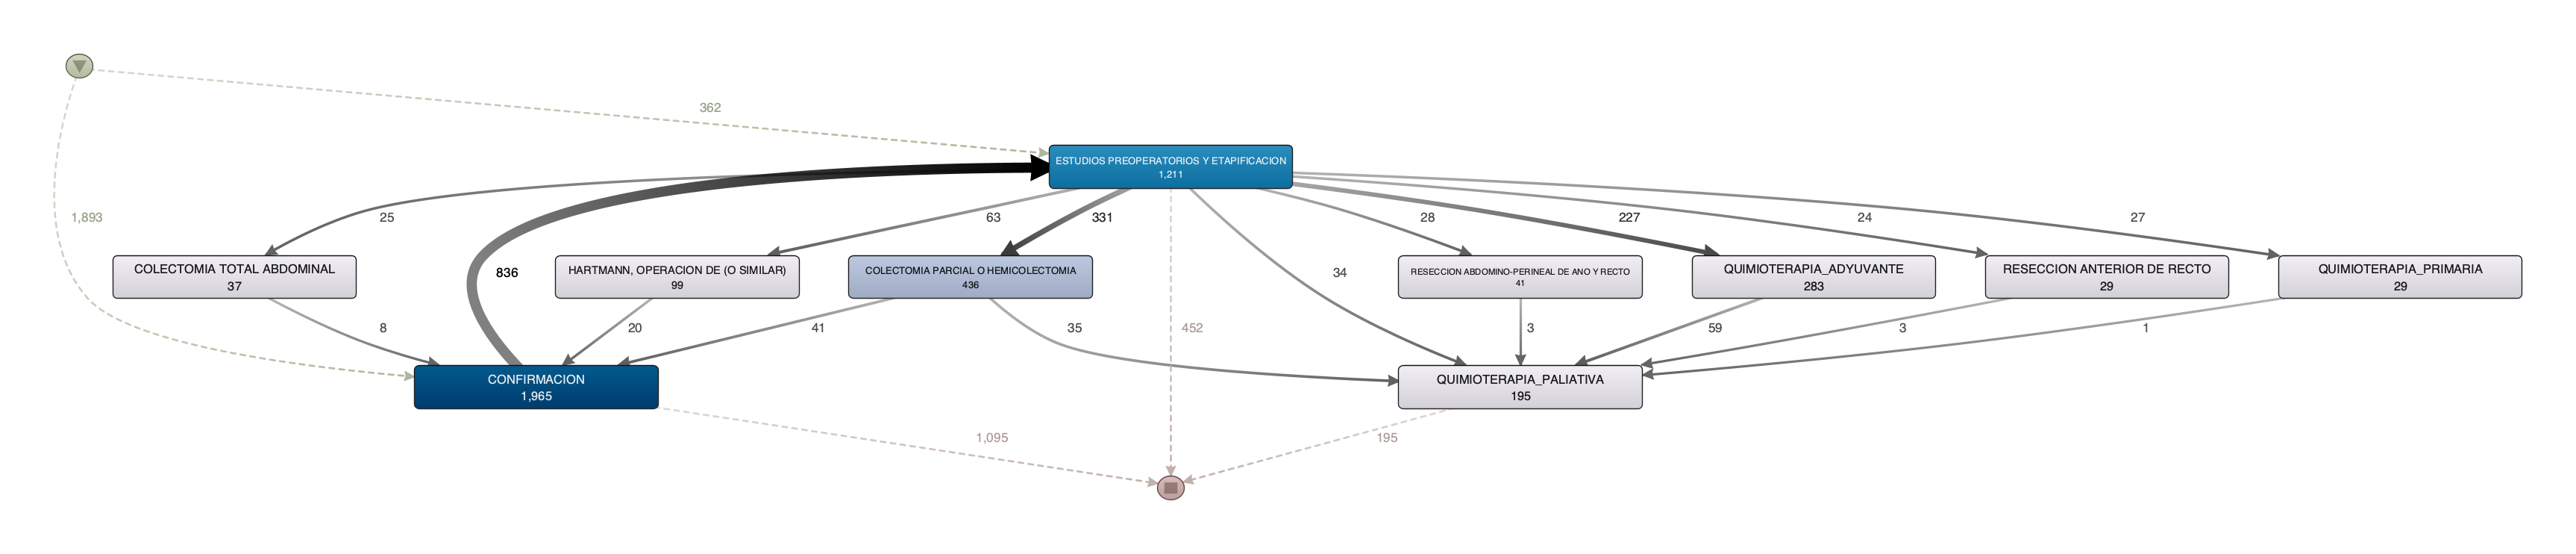
\includegraphics[width=1\textwidth]{images/3.methodology/benefits100_20.png}
    \caption{Benefits delivered to CRC Patients in Disco}
    \label{fig:benefits_in_disco}
\end{figure}

As this visual representation is difficult to analyze, the activities were reduced to 60\% and the paths were kept at 20\%.

\begin{figure}[H]
    \centering
    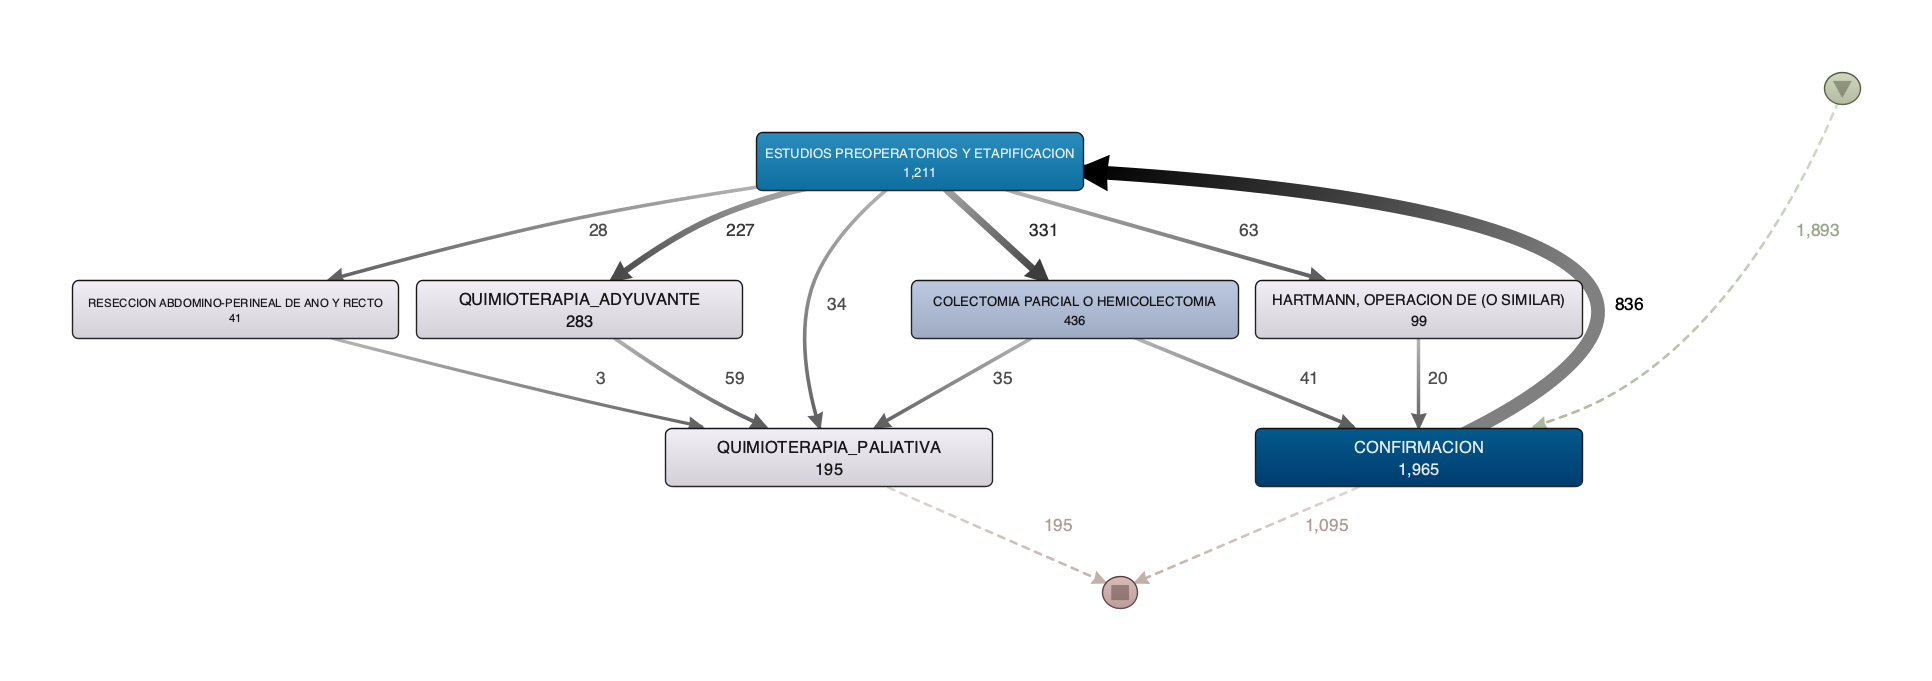
\includegraphics[width=1\textwidth]{images/3.methodology/benefits60_20.png}
    \caption{Benefits of CRC in Disco Activities at 60\% and Paths at 20\%}
    \label{fig:benefits_60_in_disco}
\end{figure}

As depicted in Figure \ref{fig:benefits_60_in_disco}, the generated process map illustrates the typical benefits received by patients undergoing CRC care. Initially, they go through the Confirmation and Staging stages, followed by receiving treatment. This treatment typically encompasses surgical interventions such as colectomy, Hartmann procedure, or abdominoperineal resection, along with adjunctive or palliative chemotherapy.

\subsection*{Insights from the MND Team}

Examining both process maps offers a glance into the prevalent pathways in CRC care. However, relying only on them offers a nearsighted picture of the current state of CRC treatment within the SMPHS. To widen our perspective into the intricacies of diagnostic and treatment processes for CRC, the insights provided by the MND team are indispensable.

The following Figure \ref{fig:process_overview} presents the diagnostic and treatment process for CRC, as viewed through the lens of the MND team:

\begin{figure}[H]
    \centering
    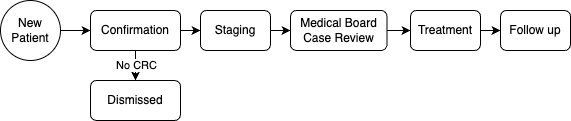
\includegraphics[width=1\textwidth]{images/3.methodology/ProcessOverview1.drawio.png}
    \caption{Process Overview according to the MND team}
    \label{fig:process_overview}
\end{figure}

Following are detailed descriptions of each process based on insights gathered from interviews with the MND team:

\begin{description}
   \item[Suspicion] A patient arrives at a public healthcare facility exhibiting symptoms suggestive of CRC, such as rectal bleeding, diarrhea, constipation, abdominal pain, weight loss, or anemia. While these symptoms may indicate other conditions, practitioners suspect CRC and refer patients to Barros Luco Hospital, the only facility equipped for colonoscopies within the Service.
   
   \item[Confirmation] Upon suspicion of CRC, patients undergo colonoscopy, with scheduling prioritized based on urgency. Some patients receive immediate scheduling, while others are placed on a waiting list. Barros Luco Hospital is the sole facility within the SMPHS equipped to perform colonoscopies, with a specialized team dedicated to this purpose.
   
   \item[Staging] Following CRC confirmation, patients undergo additional exams, including blood and imaging tests. Blood exams provide crucial insights into the patient's condition, guiding surgical decisions, while imaging tests help determine the required procedure.
   
   \item[Medical Board Review] This stage is not directly captured in the Benefits or Stages dataset. However, it plays a critical role in the treatment process. The case is presented to a Medical Board responsible for determining the most suitable treatment plan. It's important to note that not all treatments aim for a cure; some are palliative, especially for patients with advanced cancer stages. This stage begins when the results of the Staging exams are available and concludes when the board reaches a resolution.
   
   \item[Treatment] The Treatment phase begins when the Medical Board concludes its review and ends when the first treatment procedure is initiated. The treatment typically involves chemotherapy/radiotherapy and/or surgical procedures.
   
   \item[Follow-up] Following the completion of treatment, patients participate in yearly follow-up meetings for at least the next five years, or longer based on their individual circumstances.
\end{description}

This comprehensive analysis, informed by insights from the MND team, provides a detailed perspective on the CRC care process within the Service. Remarkably, certain stages are absent from the process maps. The suspicion stage is not represented due to the GES system's initiation upon suspicion, making this phase irrelevant to GES guarantees. However, the absence of metrics for the Medical Board Review stage raises concerns regarding its influence on overall process performance. Furthermore, the Follow-up stage was deliberately omitted from the data analysis due to a lack of sufficient cases, as discussed in the \hyperref[sec:data_preprocessing]{Data Preprocessing} subsection.

\subsection*{Performance Metrics}

The government has instituted specific timelines for the completion of each stage within the CRC care process by law, as outlined in Figure \ref{fig:government_kpis}. The decision to investigate this particular disease was influenced by the MND team's observation that the compliance percentage with these designated time frames consistently lagged behind for CRC. This emphasis on time frames underscores the significance of addressing potential delays in the diagnostic and treatment phases to improve overall healthcare efficiency.

\begin{figure}[H]
    \centering
    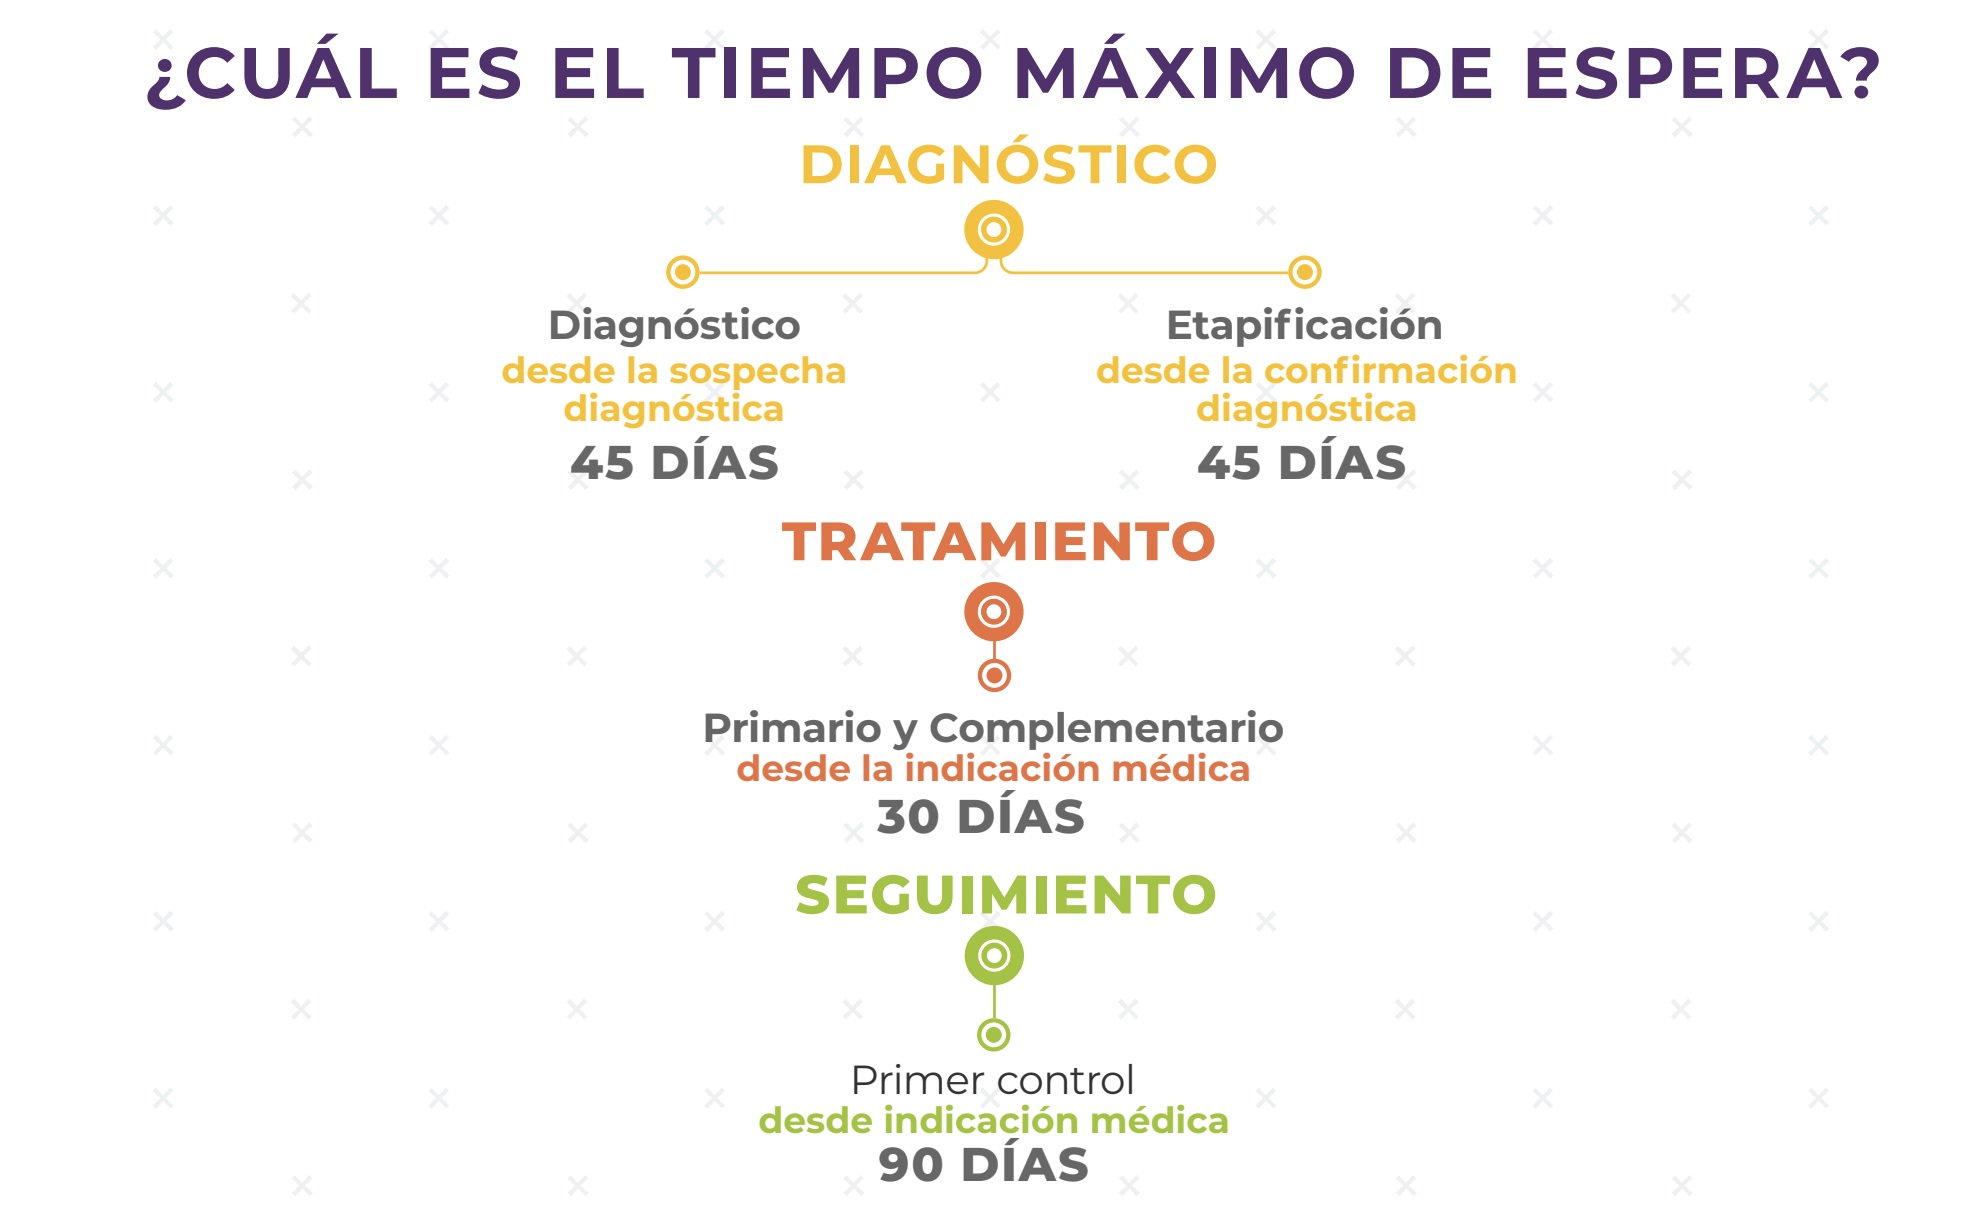
\includegraphics[width=1\textwidth]{images/3.methodology/KPIGobierno.png}
    \caption{Government-mandated stage Time Frame for CRC Diagnosis and Treatment\textsuperscript{1}}
    \label{fig:government_kpis}
\end{figure}

\footnotetext[\value{footnote}]{From \textit{Cáncer Colorectal en
Personas de 15 años y más}. Superintendencia de Salud, 2023. \url{https://www.superdesalud.gob.cl/difusion/665/articles-18886_archivo_fuente.pdf}}

Figure \ref{fig:government_kpis} illustrates the time frame requirements mandated by the government for the diagnostic phase of colorectal cancer care. Both the Confirmation and Staging stages must be completed within 45 days of the initial suspicion and diagnostic confirmation. Subsequently, treatment initiation is mandated to commence within 30 days of the medical order. Following treatment completion, the first follow-up meeting should be scheduled within 90 days.

\begin{table}[H]
\caption{Government-mandated Time Frame compliance}
\centering
\begin{tabular}{|c|c|c|}
\hline
 & N & On-time(\%)\\ \hline
Confirmation & 2552 & 1462 (57.28\%)\\ \hline
Staging &      1435 & 1204 (83.9\%)\\ \hline
Treatment &    933  & 519 (55.62\%)\\ \hline
Follow-up &    168  & 108 (64.28\%)\\ \hline
\end{tabular}
\label{table:government_kpis_compliance}
\end{table}

Table \ref{table:government_kpis_compliance} provides insights into the timeliness of CRC care stages. Notably, the Confirmation and Treatment stages consistently lag behind the designated time frames. In contrast, the Staging process generally meets the expected timelines. This highlights the need for focused efforts to improve efficiency in the Confirmation and Treatment stages, ultimately enhancing adherence to prescribed timelines and improving care for CRC patients.

\section{Process Analysis}

The process analysis builds upon the information presented in the previous section, with a distinct emphasis on the invaluable contribution of the MND team. Combining the information gathered from the understanding of the CRC care process, performance metrics, scientific research and medical advice provided enough evidence to suggest issues and a potential improvement strategy for the SMPHS.

Furthermore, the collaborative approach aims to guarantee that the proposed improvements are not only identified accurately but are also pragmatic in terms of implementation difficulty and the available resources. This collaborative perspective enriches the process analysis, aligning it with the identified challenges and offering feasible solutions within the context of the Southern Metropolitan district's healthcare system.

\subsection*{Current Issues}

This research stage was approached with care due to the little experience the investigator had in the medical and operational field. Every idea that came up was discussed with the MND team to validate if it was indeed an issue for the SMPHS.

\subsubsection*{Poor Performance in the Confirmation Stage}

Figure \ref{fig:confirmation_stage} displays the Stages process map, isolating the cases where the Confirmation activity is involved. One notaworthy observation from this analysis is the significant proportion of patients progressing only through the Confirmation stage. As depicted in the "CONFIRMATION" activity in Figure \ref{fig:confirmation_stage}, approximately 56.4\% of patients exit the CRC care process after Confirmation. This departure should mostly be attributed to negative colonoscopy results. However, this trend may indicate data incompleteness, particularly in the cases where patients transition from the "CONFIRMATION" activity to "PASSING CAUSED BY CRC", creating uncertainty about their treatment status. These patients likely received a positive CRC result but may have opted for treatment in the private sector or no treatment at all.

\begin{figure}[H]
    \centering
    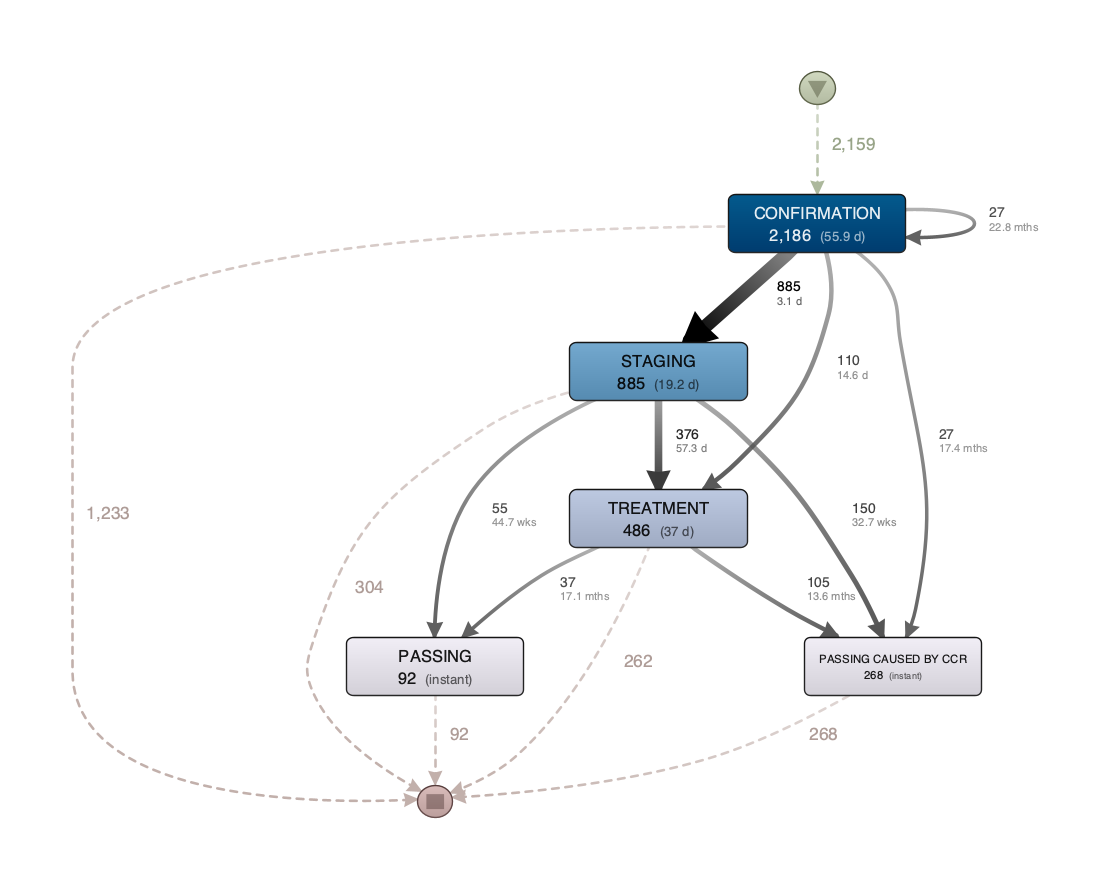
\includegraphics[width=1\textwidth]{images/3.methodology/confirmation_stage.png}
    \caption{Confirmation Stage in Disco}
    \label{fig:confirmation_stage}
\end{figure}

As shown in Table \ref{table:government_kpis_compliance}, a notable concern regarding the Confirmation stage is that only 57.28\% of confirmations occur within the prescribed time frame. Furthermore, as illustrated in the "CONFIRMATION" activity on Figure \ref{fig:confirmation_stage}, the average waiting time for CRC diagnosis confirmation extends to 55.9 days. 

\begin{figure}[H]
    \centering
    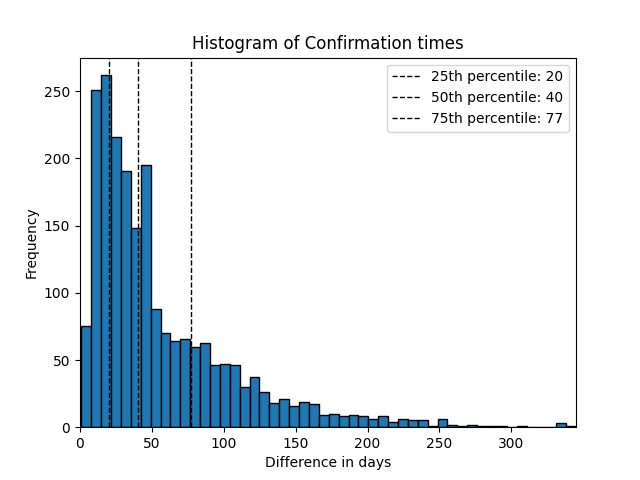
\includegraphics[width=1\textwidth]{images/3.methodology/confirmation_histogram.png}
    \caption{Confirmation Histogram}
    \label{fig:confirmation_histogram}
\end{figure}

In Figure \ref{fig:confirmation_histogram}, we observe that a quarter of patients receive their confirmation results in 20 days or less, while another quarter wait for more than 77 days. While this duration may not significantly affect disease progression given CRC's long sojourn time, it undoubtedly causes discomfort for patients and their families.

Given this performance, one has to consider the colonoscopy capacity of the SMPHS. In 2020, the population of the Netherlands was approximately 17.4 million people, and the number of colonoscopies performed was 44,036 \cite{noauthor_national_nodate}. This translates to 0.0025 colonoscopies per person. Considering that the Netherlands has one of the best healthcare systems for CRC prevention \cite{navarro_colorectal_2017}, the SMPHS, with a population of approximately 1.1 million, should be performing 2,750 colonoscopies every year. However, based on the Stages dataset covering about 4.85 years, the SMPHS is currently performing approximately 526 colonoscopies annually.

Beyond its potential impact on disease management, this observed pattern is indicative of the current confirmation stage performance. Most patients receive confirmation results after a prolonged period following CRC suspicion, likely due to limited resources for coloscopy procedures. This prolonged waiting period affects patient morale and their readiness to undergo future diagnostic and treatment procedures critical to their overall well-being.

\subsubsection*{Missing treatments}

Figure \ref{fig:staging_stage} displays the Stages process map, isolating the cases where the Staging activity is involved. A notable trend from previous chapters is the significant number of patients who discontinue their progression through the CRC care process, particularly after the Confirmation and Staging activities. As depicted in the "STAGING" activity of Figure \ref{fig:confirmation_stage}, only 376 out of 885 individuals (42.49\%) who completed both activities received treatment in the public sector. Similarly, in Figure \ref{fig:staging_stage}, only 511 out of 1250 individuals (40.88\%) who went through the "STAGING" activity continued with the "TREATMENT" activity.

\begin{figure}[H]
    \centering
    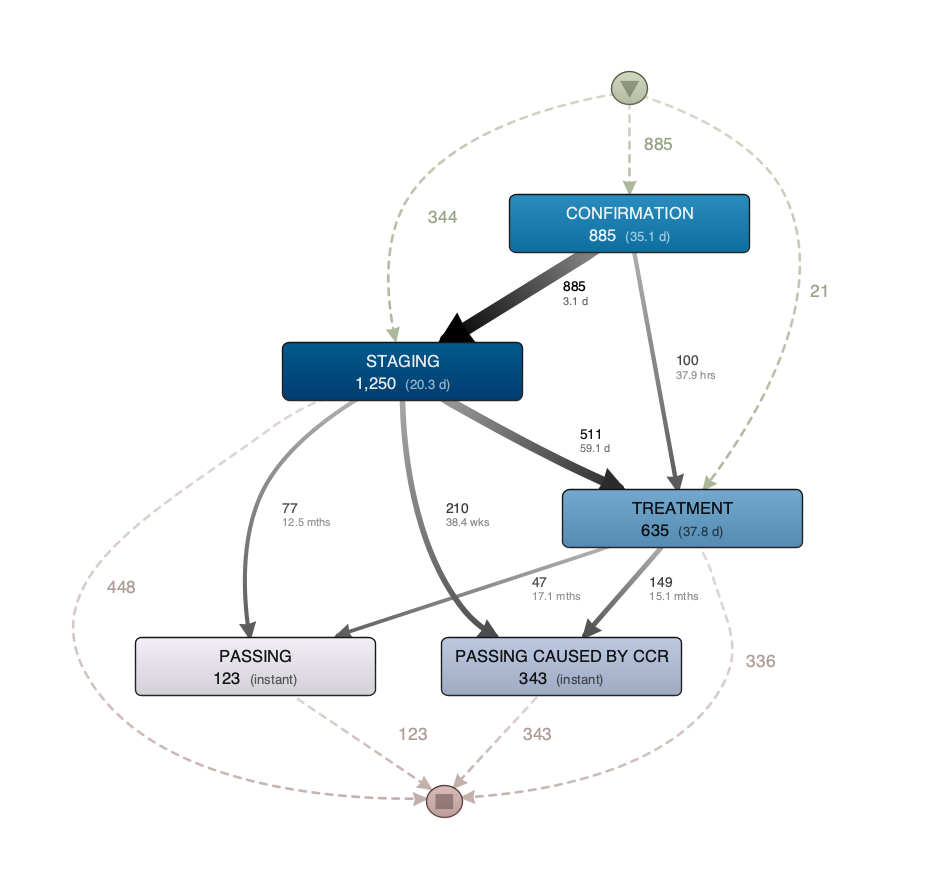
\includegraphics[width=1\textwidth]{images/3.methodology/staging_stage.png}
    \caption{Staging Stage in Disco}
    \label{fig:staging_stage}
\end{figure}

This concerning trend highlights the public sector's struggle to deliver timely and efficient treatment, emphasizing the pressing need to improve the healthcare system's responsiveness. The harsh reality is that a considerable number of patients are opting to halt their treatment for reasons yet to be determined.

Figure \ref{fig:complete cases} shows a process map where the only cases that were kept where those were the starting activity was "CONFIRMATION" and their end activity was either "TREATMENT", "PASSING" or "PASSING CAUSED BY CRC".

\begin{figure}[H]
    \centering
    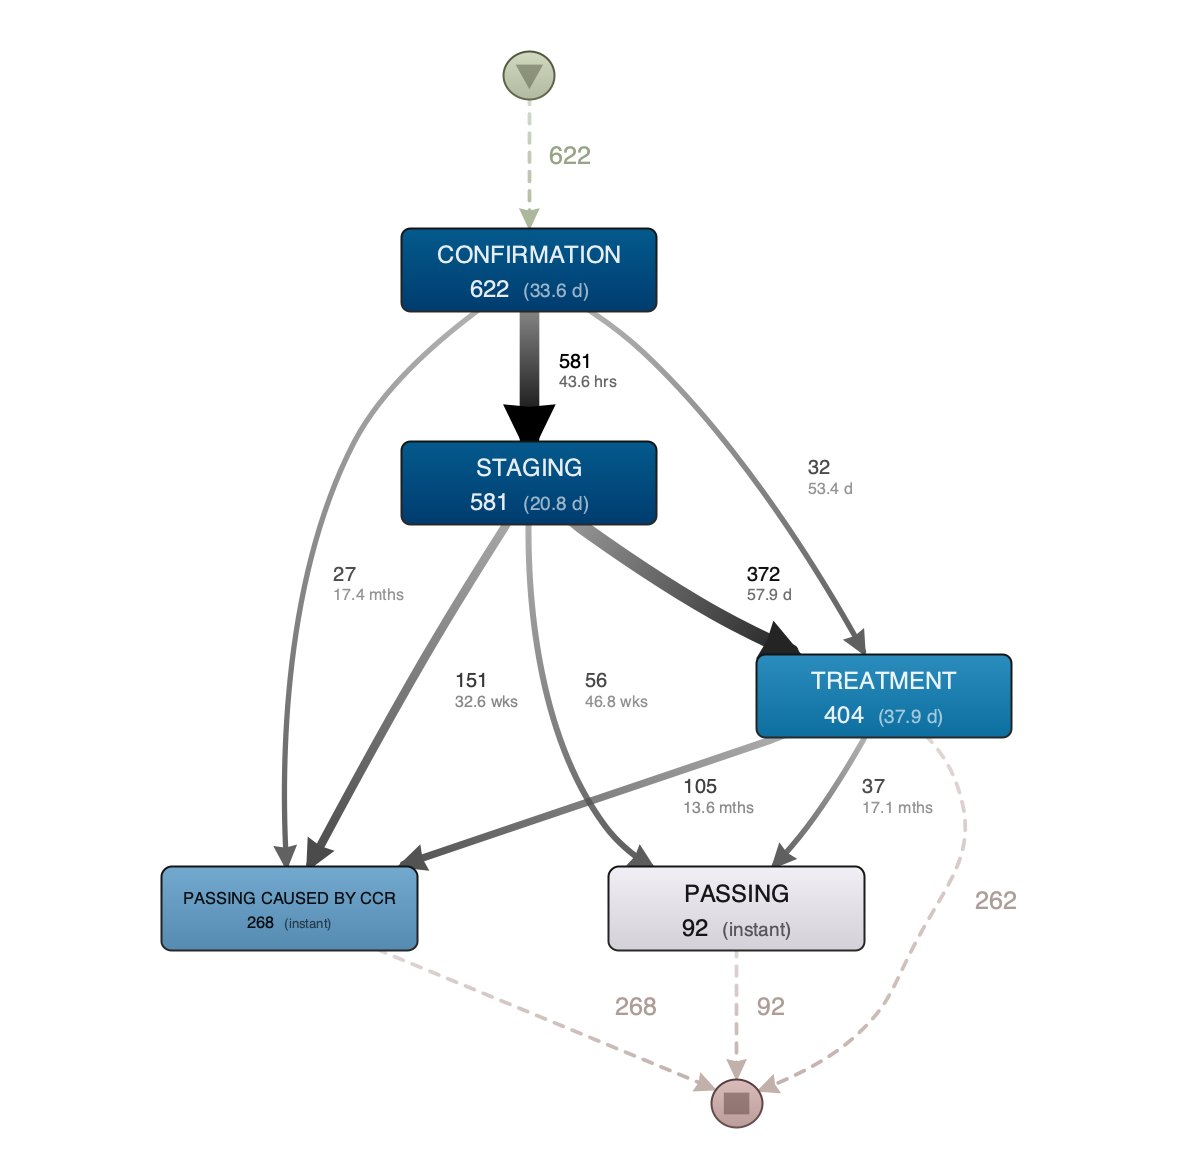
\includegraphics[width=1\textwidth]{images/3.methodology/complete_cases.png}
    \caption{Complete Cases in Disco}
    \label{fig:complete cases}
\end{figure}

It's worth noting that, on average, the sum of waiting times across all activities preceding the start of treatment ("CONFIRMATION", "STAGING" and "TREATMENT" amounts to 152 days (33.6+1.8+20.8+57.9+37.9), roughly equivalent to 5 months from the initial suspicion to treatment commencement. This prolonged timeline highlights the urgent need for expedite access to treatment within the public sector to improve outcomes and reduce the risks associated with delayed intervention.

\subsubsection*{Lack of preventive medicine}

A key insight, emphasized by both the MND team and supported by the literature review, is the importance of preventive medicine in the Chilean public healthcare system. According to a survey conducted in Chile with 1893 respondents, as reported by \citeA{alfaro_barriers_2024}, 79.6\% of the respondents stated they had never undergone any form of CRC screening, and 90.4\% had not been screened for CRC in the last three years.  Interestingly, among respondents with private insurance (26.8\% of the total), screening rates were better, indicating a potentially even worse situation within the SMPHS.

This data implies that nearly all patients seeking care within the public sector are diagnosed as symptomatic patients, meaning their diagnosis occurred after they had already exhibited signs of the suspected disease. It is widely agreed among researchers that implementing screening methods is a critical step toward improving the prognosis for CRC patients \cite{van_rossum_earlier_2009, soerjomataram_most_2012}.

\begin{figure}[H]
    \centering
    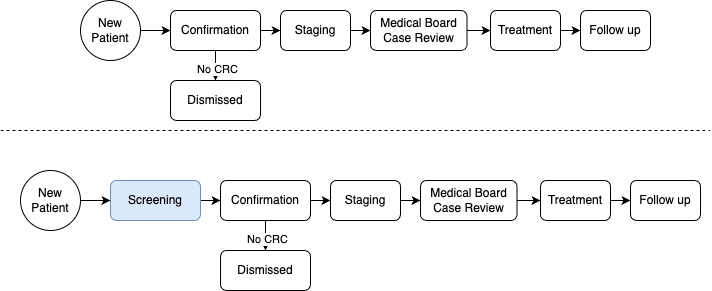
\includegraphics[width=1\textwidth]{images/3.methodology/ProcessOverview2.drawio.png}
    \caption{Diagnosing and treating patients with Screening Stage}
    \label{fig:process_overview_2}
\end{figure}

Figure \ref{fig:process_overview_2} depicts the Process Overview with an additional Screening activity. Currently, the most effective screening methods involve detecting blood in fecal matter, with widely used tests like the fecal occult blood test (FOBT) and the fecal immunochemical test (FIT) showing consistent improvement over the years. These tests have been successfully integrated into numerous public healthcare systems, most of them from Europe \cite{navarro_colorectal_2017}. 

Most preventive strategies revolve around using these exams to determine eligibility for periodic preventive colonoscopies, offering the tests annually. Some strategies also consider providing preventive colonoscopies every five or ten years, but this approach is often considered expensive due to the increased number of required colonoscopies resulting from false positives. The majority of researched strategies recommend initiating these screenings at age 50.

Compelling evidence suggests that implementing these preventive strategies can lead to cost savings in certain scenarios \cite{lansdorp-vogelaar_effect_2009}. This cost-saving effect is primarily attributed to the early detection of cancerous tumors at an asymptomatic stage, which results in less advanced disease and subsequently reduces the costs associated with treatment. Nonetheless, a major challenge remains in persuading the population to undergo regular preventive screenings, thereby promoting early detection and intervention.

\subsection*{Potential Improvement Strategy}

Crafting an effective improvement strategy poses a formidable challenge, particularly given that the main issues can be summarized as a process with poor time delivery performance. This means that there is not a clear path for improvement but the objective is to streamline the delivery of diagnosis results and treatments. The complexity intensifies as the resources for the SMPHS are limited, therefore any increase in the CRC care budget has to be properly justified. 

The delayed Confirmation and Treatment stages reveal the overburden of the SMPHS in the CRC care process. It is unclear whether the care units involved need more resources or if the optimization of existing resources is required. However, it is evident that both are failing to meet their objectives on time.

Addressing the issue of missing treatments is crucial for the improvement strategy, as it strongly suggests dissatisfaction with the public healthcare system's performance. To rectify this, one of the strategy's most important objectives must be to enhance the overall performance of the diagnostic and treatment process, instilling confidence in patients to continue treatment within the public healthcare system.

Considering the lack of preventive medicine, the poor performance of the CRC care process and the advice of the MND team, the implementation of a Screening stage emerges as a valid proposal for an improvement strategy. This reallocation of resources from treatments to diagnosis can improve CRC prognosis and potentially result in cost savings. However, it's important to note that this strategy does not directly address the main issues currently affecting the SMPHS's CRC care process, which are primarily related to a lack of resources and/or inefficient use of them.

The subsequent chapters will simulate and calculate the potential costs and benefits associated with implementing a Screening stage in the current CRC care process of the SMPHS.

